\chapter{Experiments and Results}
\label{AER}

In the following section I will apply the software to demonstrate the predicted dynamics of the phages and bacteria under different conditions. 
I first begin with analyzing the model using a Sobol analysis on the simple Golding model, \Cref{eq:golding_model}. 
Using the most important parameters identified from the Sobol analysis, I run multiple IVAs to describe the change in graph behavior for different inputs. 
I use the information gained from this to describe how the graphs change for a wide range of inputs. 
Next, I analyze if phages will proliferate or not depending on the initial phage, uninfected bacteria, and resource concentration. 
I finally extend the analyses to a large community and analyze how changing parameter values will change the phage and bacteria growth, and if the phages and bacteria can coexist or not. 

\section{A Realistic Growth Curve}
As the bacterial population grows, resource consumption accelerates until only trace amounts remain. 
The delay between the peaks of uninfected and infected bacteria is due to the infection stages and the latent period of phage infection. 
Each bacterium transitions from infection stage $k$ to $k+1$ at a rate of $\frac{M}{\tau}$. 
Therefore, decreasing the number of infection steps $M$ or increasing the latent period $\tau$ amplifies this delay. 
A longer latent period means it takes more time for bacteria to progress through the infection stages.

At $t=4$, the infection rate surpasses the bacterial replication rate, causing the bacterial population to decline even though resources are still available. 
This moment coincides with the rise of the phage population. 
Observing the timing of these events and changes in the graph's behavior, as well as their relationships across different graphs, helps clarify the complex population dynamics and the interdependence of the populations. 
The nature of the models being nonlinear makes the analysis harder to understand and conceptualize. 

Understanding the system becomes more complicated as the model increases from a $1\times1\times1$ system to a $p\times b\times r$ system. 
Now up to any number of phages can interact with any number of bacteria, and any number of bacteria can interact with any number of resources, each with their own unique parameter values. 
These varying rates will significantly influence the dynamics of the system, and make it hard to determine what event caused what due to the rise in number of interactions.
There are only 2 interactions that occur in a $1\times1\times1$ system. 
With a $p\times b\times r$ system, there are at most $p\cdot b + b\cdot r$ interactions that can occur. 
So many individual events occurring at the same time makes it harder to identify the cause of the event, and how the event's action will propagate through the network. 
A method to circumvent this issue is by knocking out certain nodes or edges and rerunning the simulation and compare the results. 
The knocked out node or edge won't contribute to the simulation anymore, so there will be a cascading effect on the other populations. 
\citet{hsuDynamicModulationGut2019} found that predating a specific bacteria strain in a mouse's gut microbiome with a phage had a cascading effect in other bacteria populations due to interbacterial interactions. 

\section{Sobol Sensitivity Analysis Results}
\label{sec:Sobol_sensitivity_analysis_results}
The Sobol method is a global sensitivity analysis technique that quantifies the contribution of each input parameter, as well as their interactions, to the variance of a model's univariate output. 
It decomposes the output variance into fractions attributed to individual parameters and their combinations, providing first-order and total-order sensitivity indices.
A Sobol analysis identifies the most influential parameters affecting model output. 
The insights from this analysis inform the selection of key parameters for subsequent simulations, ensuring that further investigations focus on those with the greatest impact.

\Cref{fig:created:Sobol_final_no_wi_wo} shows the impact that the parameter had on the final value of the population at $t=15$ for a $1\times 1\times 1$ system, on the original Golding model, \Cref{eq:golding_model}. 
\Cref{fig:created:Sobol_peak_no_wi_wo} shows the impact that the parameter had on the peak population count, using the 95\% rule. 
\Cref{fig:created:Sobol_peak_time_no_wi_wo} shows the impact that the parameter had on the time of the peak, using the 95\% rule. 

The parameters that were tested include all the parameters listed in the basic Golding model, except for the uninfected bacteria $(I_1, \dots, I_4), M, \omega^i,$ and $\omega^o$. 
Infected bacteria $I_k$ was not included as it doesn't make sense to start with infected bacteria to the system. 
$M$, the number of stages that the infection goes through, can not be tested with Sobol as $M$ is an integer, while Sobol randomly chooses float values. 
While testing, the washin rate $\omega^i$ and washout rate $\omega^o$ consistently had the largest influence on the final, peak value, and time of peak value, using the 95\% rule. 
Washin and washout are not part of the original model from Golding, and the addition of a washin and washout term significantly skews the results and analysis, so it was left out of the analysis. 
The results for a Sobol analysis with washin and washout can be found in \Cref{sec:AppendixF:sobol_analysis_with_washin_and_washout}. 

\subsection{Resources}
The final value for the resources depended heavily on the initial resource concentration. 
There weren't many interactions with other parameters because $ST \gg S1$. 
$e$, the ability for the bacteria to consume resources, had little influence on the system despite $e$ acting as the link between the resources and bacteria and directly controlling the rate of resource consumption. 
$\tau$, the latent period, had a larger influence in the final resource value than $e$. 

The peak value and time of peak value graphs are empty for the Sobol indices for Resources as the resource concentration is always decreasing from different initial conditions, the initial resource always had a peak at $t=0$. 

\subsection{Phages}
The final phage population value depended on $r$ (the probability of a successful phage-bacteria infection) the most, with $\beta$ (the burst size) as the second most important parameter influencing the final population value. 
The other parameters had little to no influence on the final phage population levels. 

The Sobol peak value plot is basically the same as the final population value. 
Similar to the final value, the phage max value is highly dependent on the value of $r$ and $\beta$, and the other parameters had little to no influence on the peak value for the phages. 

For the time of peak value, $\tau$ becomes the most important parameter for determining the time of peak value, while $r$ isn't as important anymore. 
The initial phage population has a small influence on the final population value, about as equally important as $r$. 
$\beta$ roughly maintains the same sensitivity value across the final, peak, and time of peak analyses. 

\subsection{Total Bacteria}
The final total bacteria population depended mostly on $\beta$, the burst size of the phage, but via many second or there are many higher order interactions occurring as $ST \gg S1$. 
The final population depended heavily on many higher order interactions with the initial resource concentration, $\tau$, and $e$. 

$\beta$ is still the most important parameter to the model, but instead of $ST$ and $S1$ being equal to 1 and 0.28 like in the final value, the sensitivity value is only 0.54 and 0.16 respectively. 
Every parameter plays some influence on the output, but with higher order interactions as for all parameter inputs, $ST > S1$. 

$\beta$ and $\tau$ are the two most important factors in determining the time of peak for the total bacteria. 
The only parameter that does not influence the time of peak in some manner is $e$, otherwise every parameter has some sort of influence on the time at which the bacteria population peaks. 

\subsection{Results}
Some results are surprising. 
$e$, $v$ (max growth velocity of a bacteria), and $K$ (half saturation Monod constant) are consistently the least important factor in determining the final value, peak value, and time of peak. 
It would be expected that changing the parameter values that directly affect the bacterial growth would have a large impact on the resources and phages. 
More bacteria mean more resources are consumed, and more phages are created. 
Knowing that $e$, $v$, and $K$ are relatively unimportant compared to a parameter like $r$ or $\tau$, future analyses do not have to focus on $e$, $v$, and $K$. 
As $\beta$, $r$, and $\tau$ are relatively important, future analyses could focus on how those parameters influence the growth of phages and bacteria. 

\begin{figure}[ht!]
    \centering
    \begin{subfigure}{0.32\linewidth}
        \centering
        \captionsetup{width=1\linewidth}
        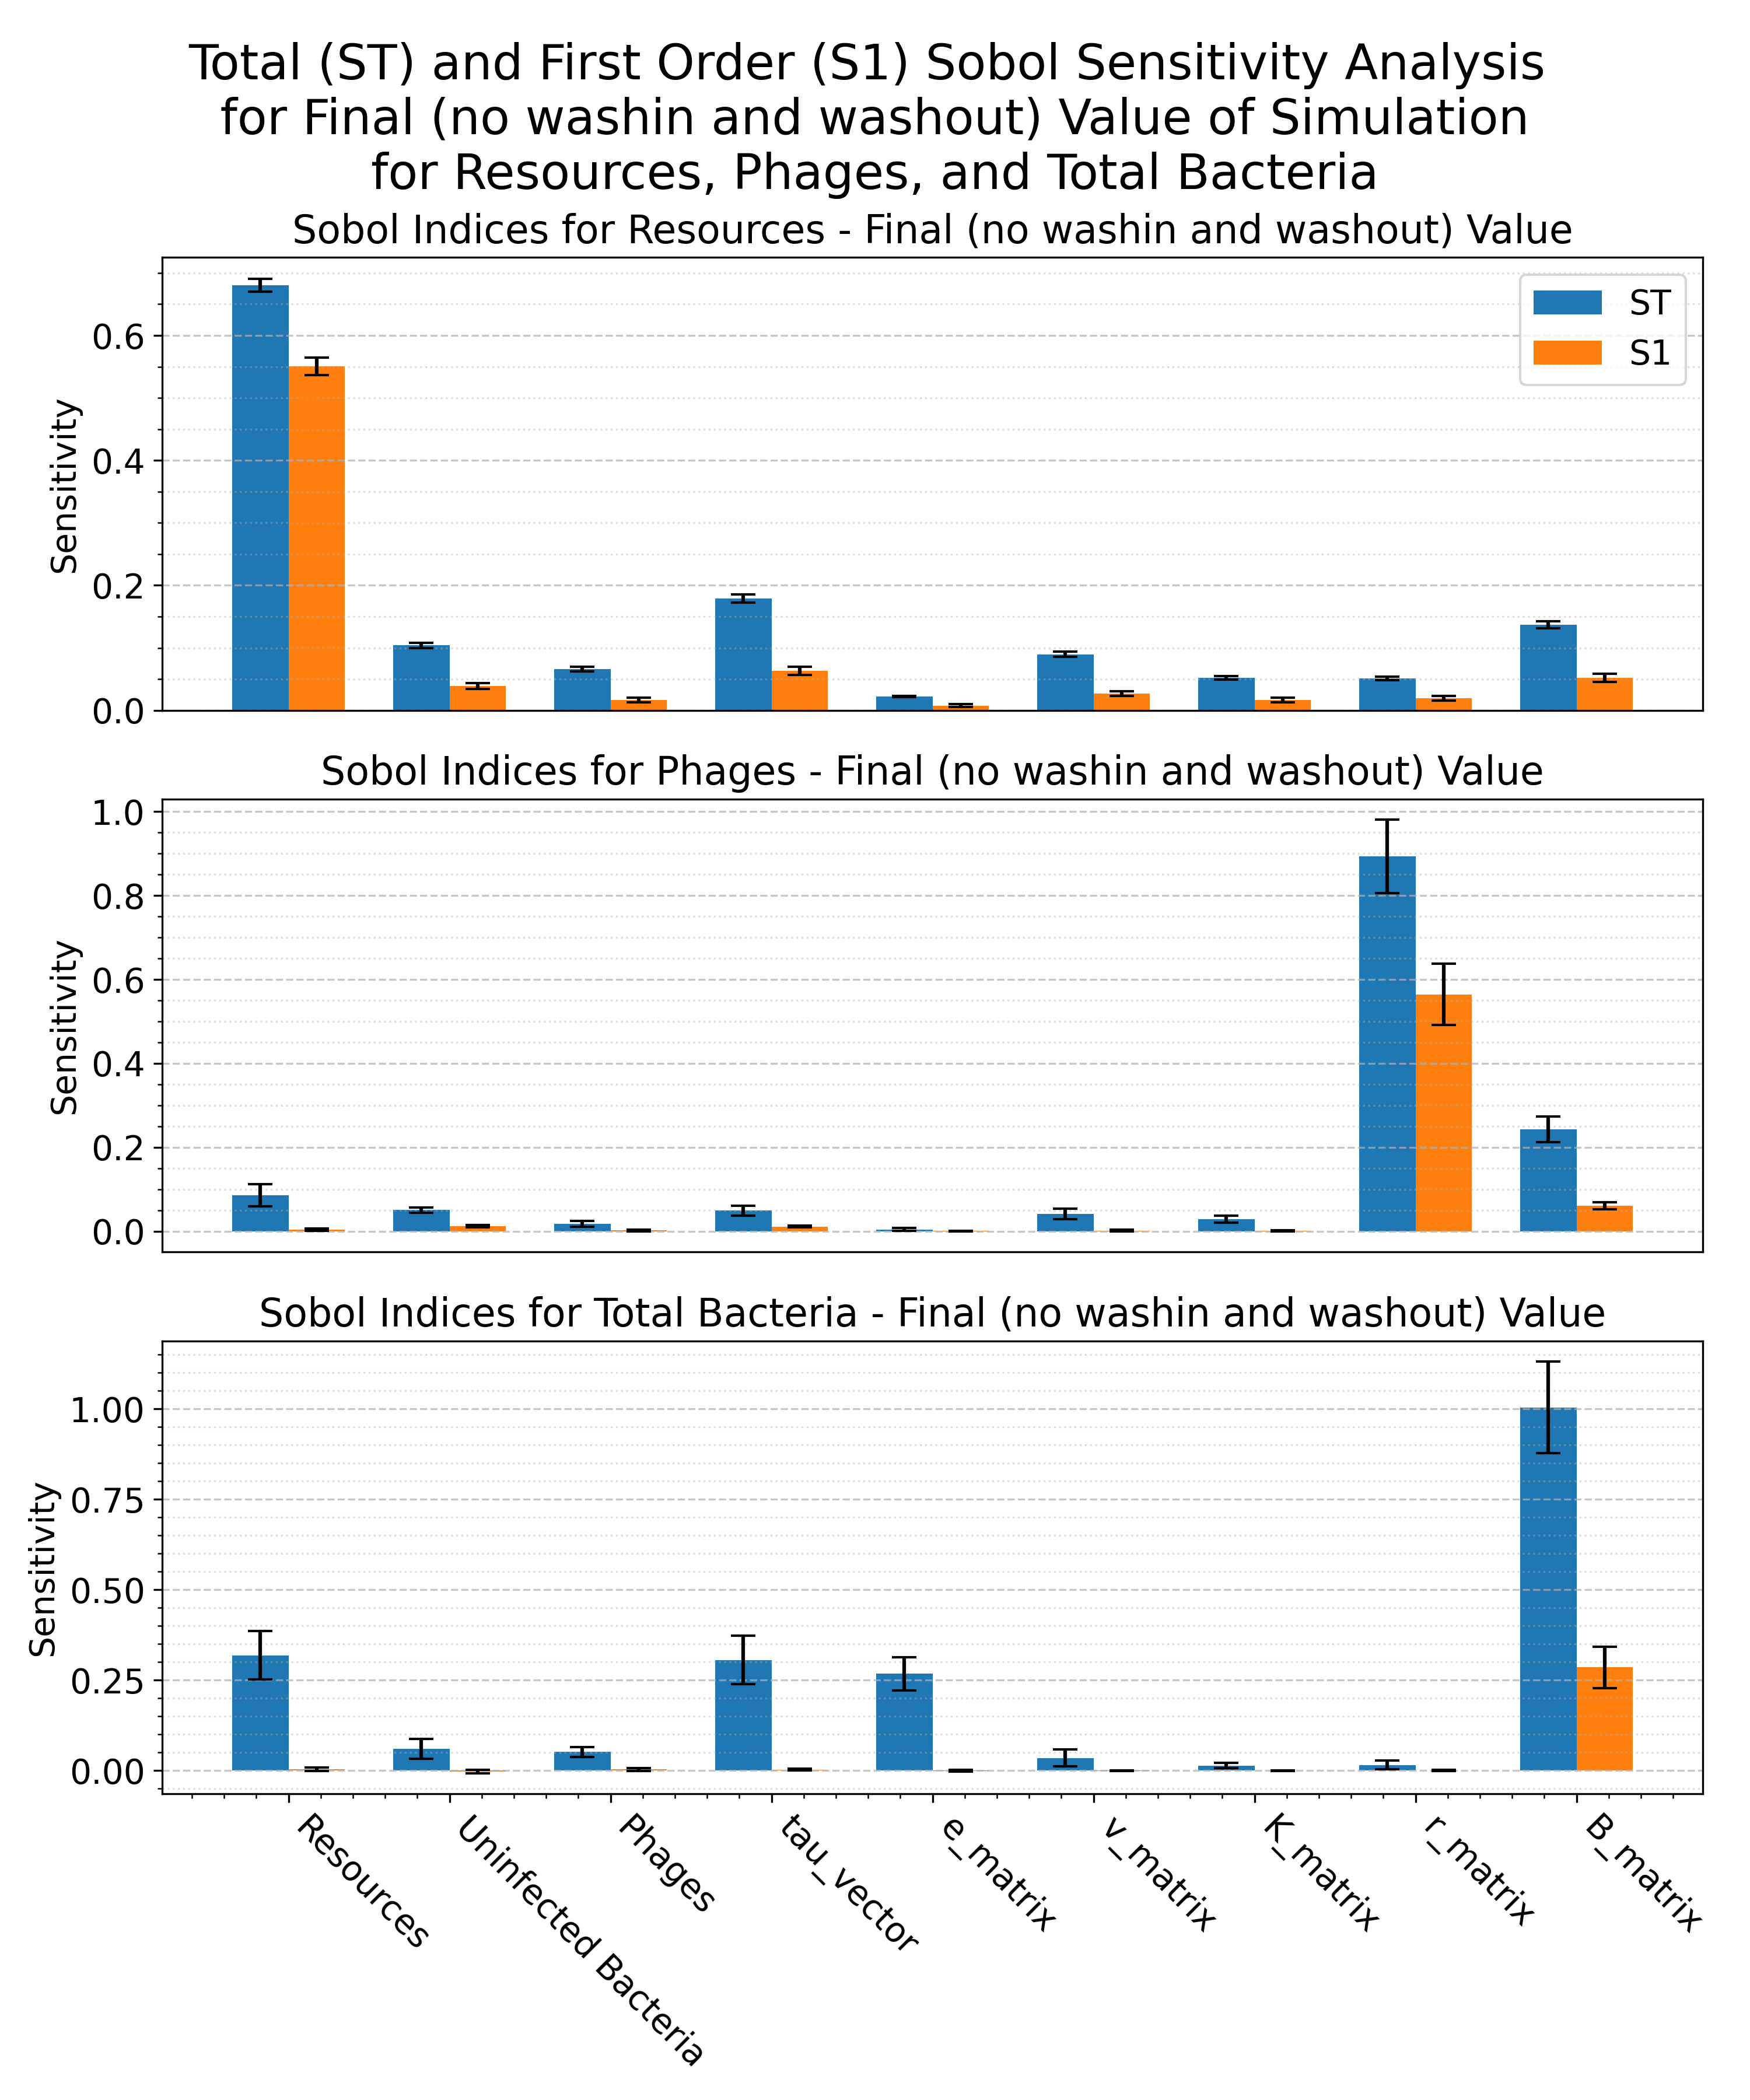
\includegraphics[width=\linewidth]{Plots/Created/SOBOL/SOBOL_analysis_1749708738_Final_(no_washin_and_washout).png}
        \caption{
            Final value, no washin and washout. 
        }
        \label{fig:created:Sobol_final_no_wi_wo}
    \end{subfigure}
    \hfill
    \begin{subfigure}{0.32\linewidth}
        \centering
        \captionsetup{width=1\linewidth}
        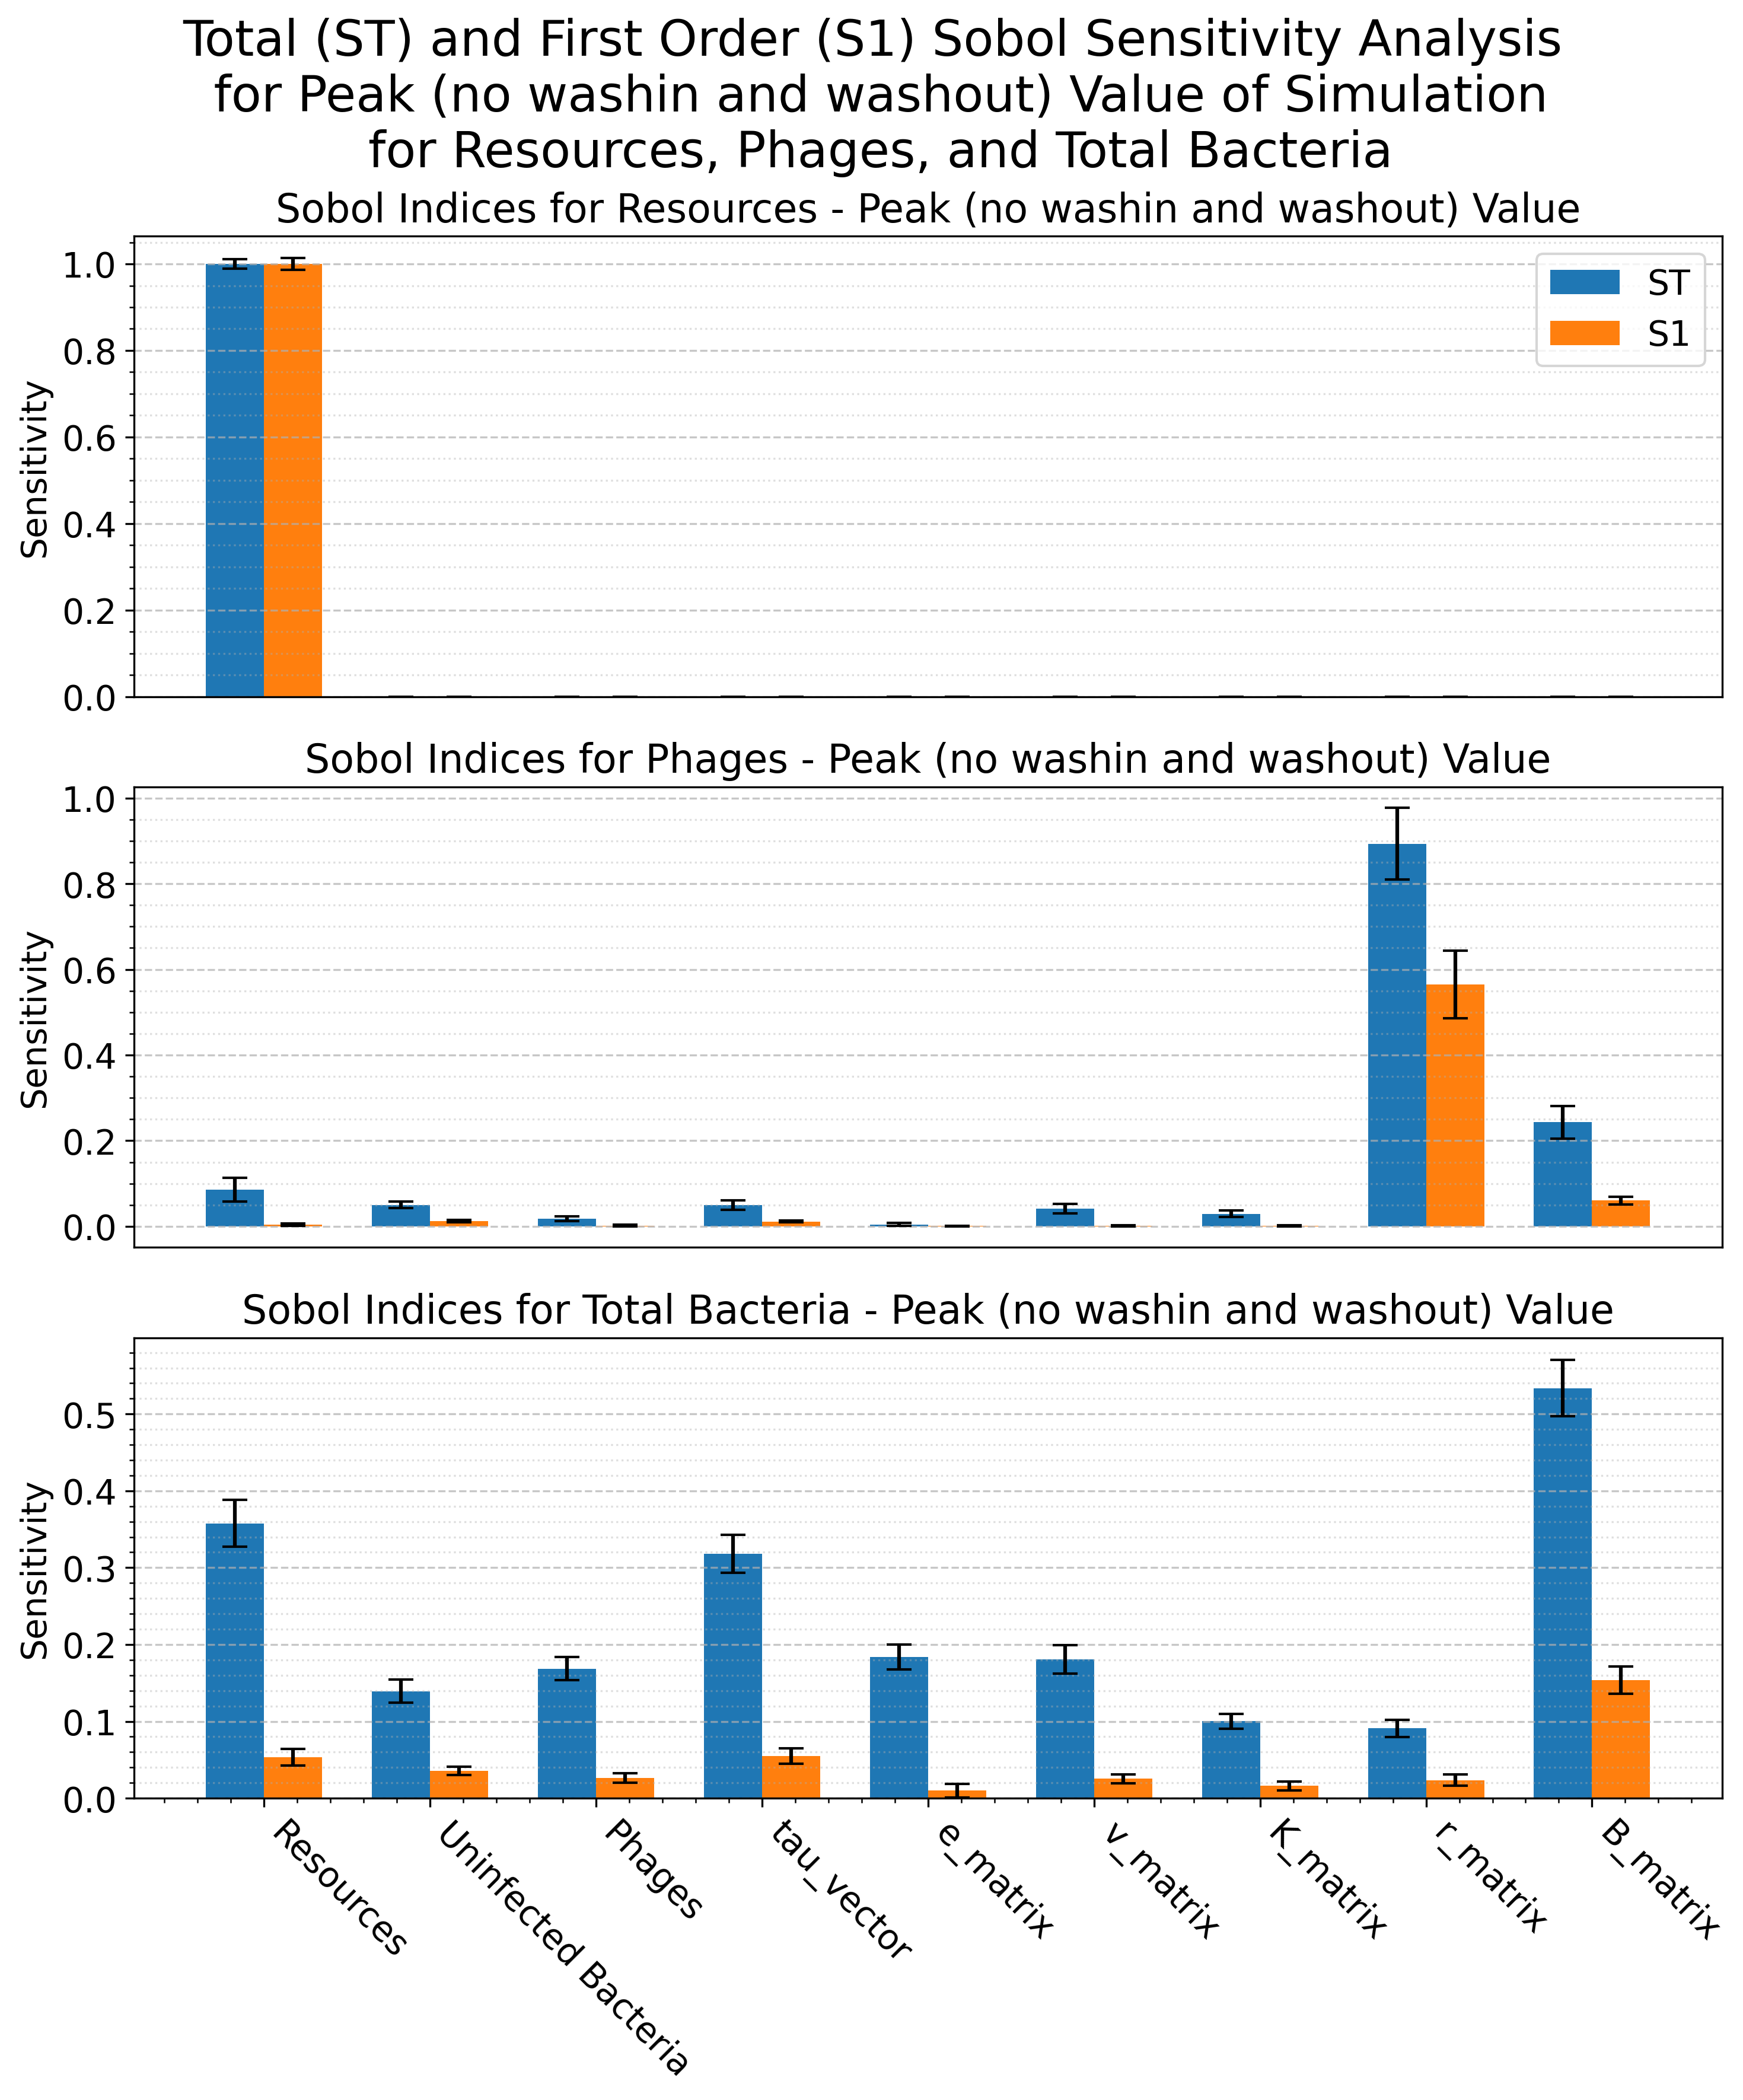
\includegraphics[width=\linewidth]{Plots/Created/SOBOL/SOBOL_analysis_1749708738_Peak_(no_washin_and_washout).png}
        \caption{
            Peak population value, no washin and washout. 
        }
        \label{fig:created:Sobol_peak_no_wi_wo}
    \end{subfigure}
    \hfill
    \begin{subfigure}{0.32\linewidth}
        \centering
        \captionsetup{width=1\linewidth}
        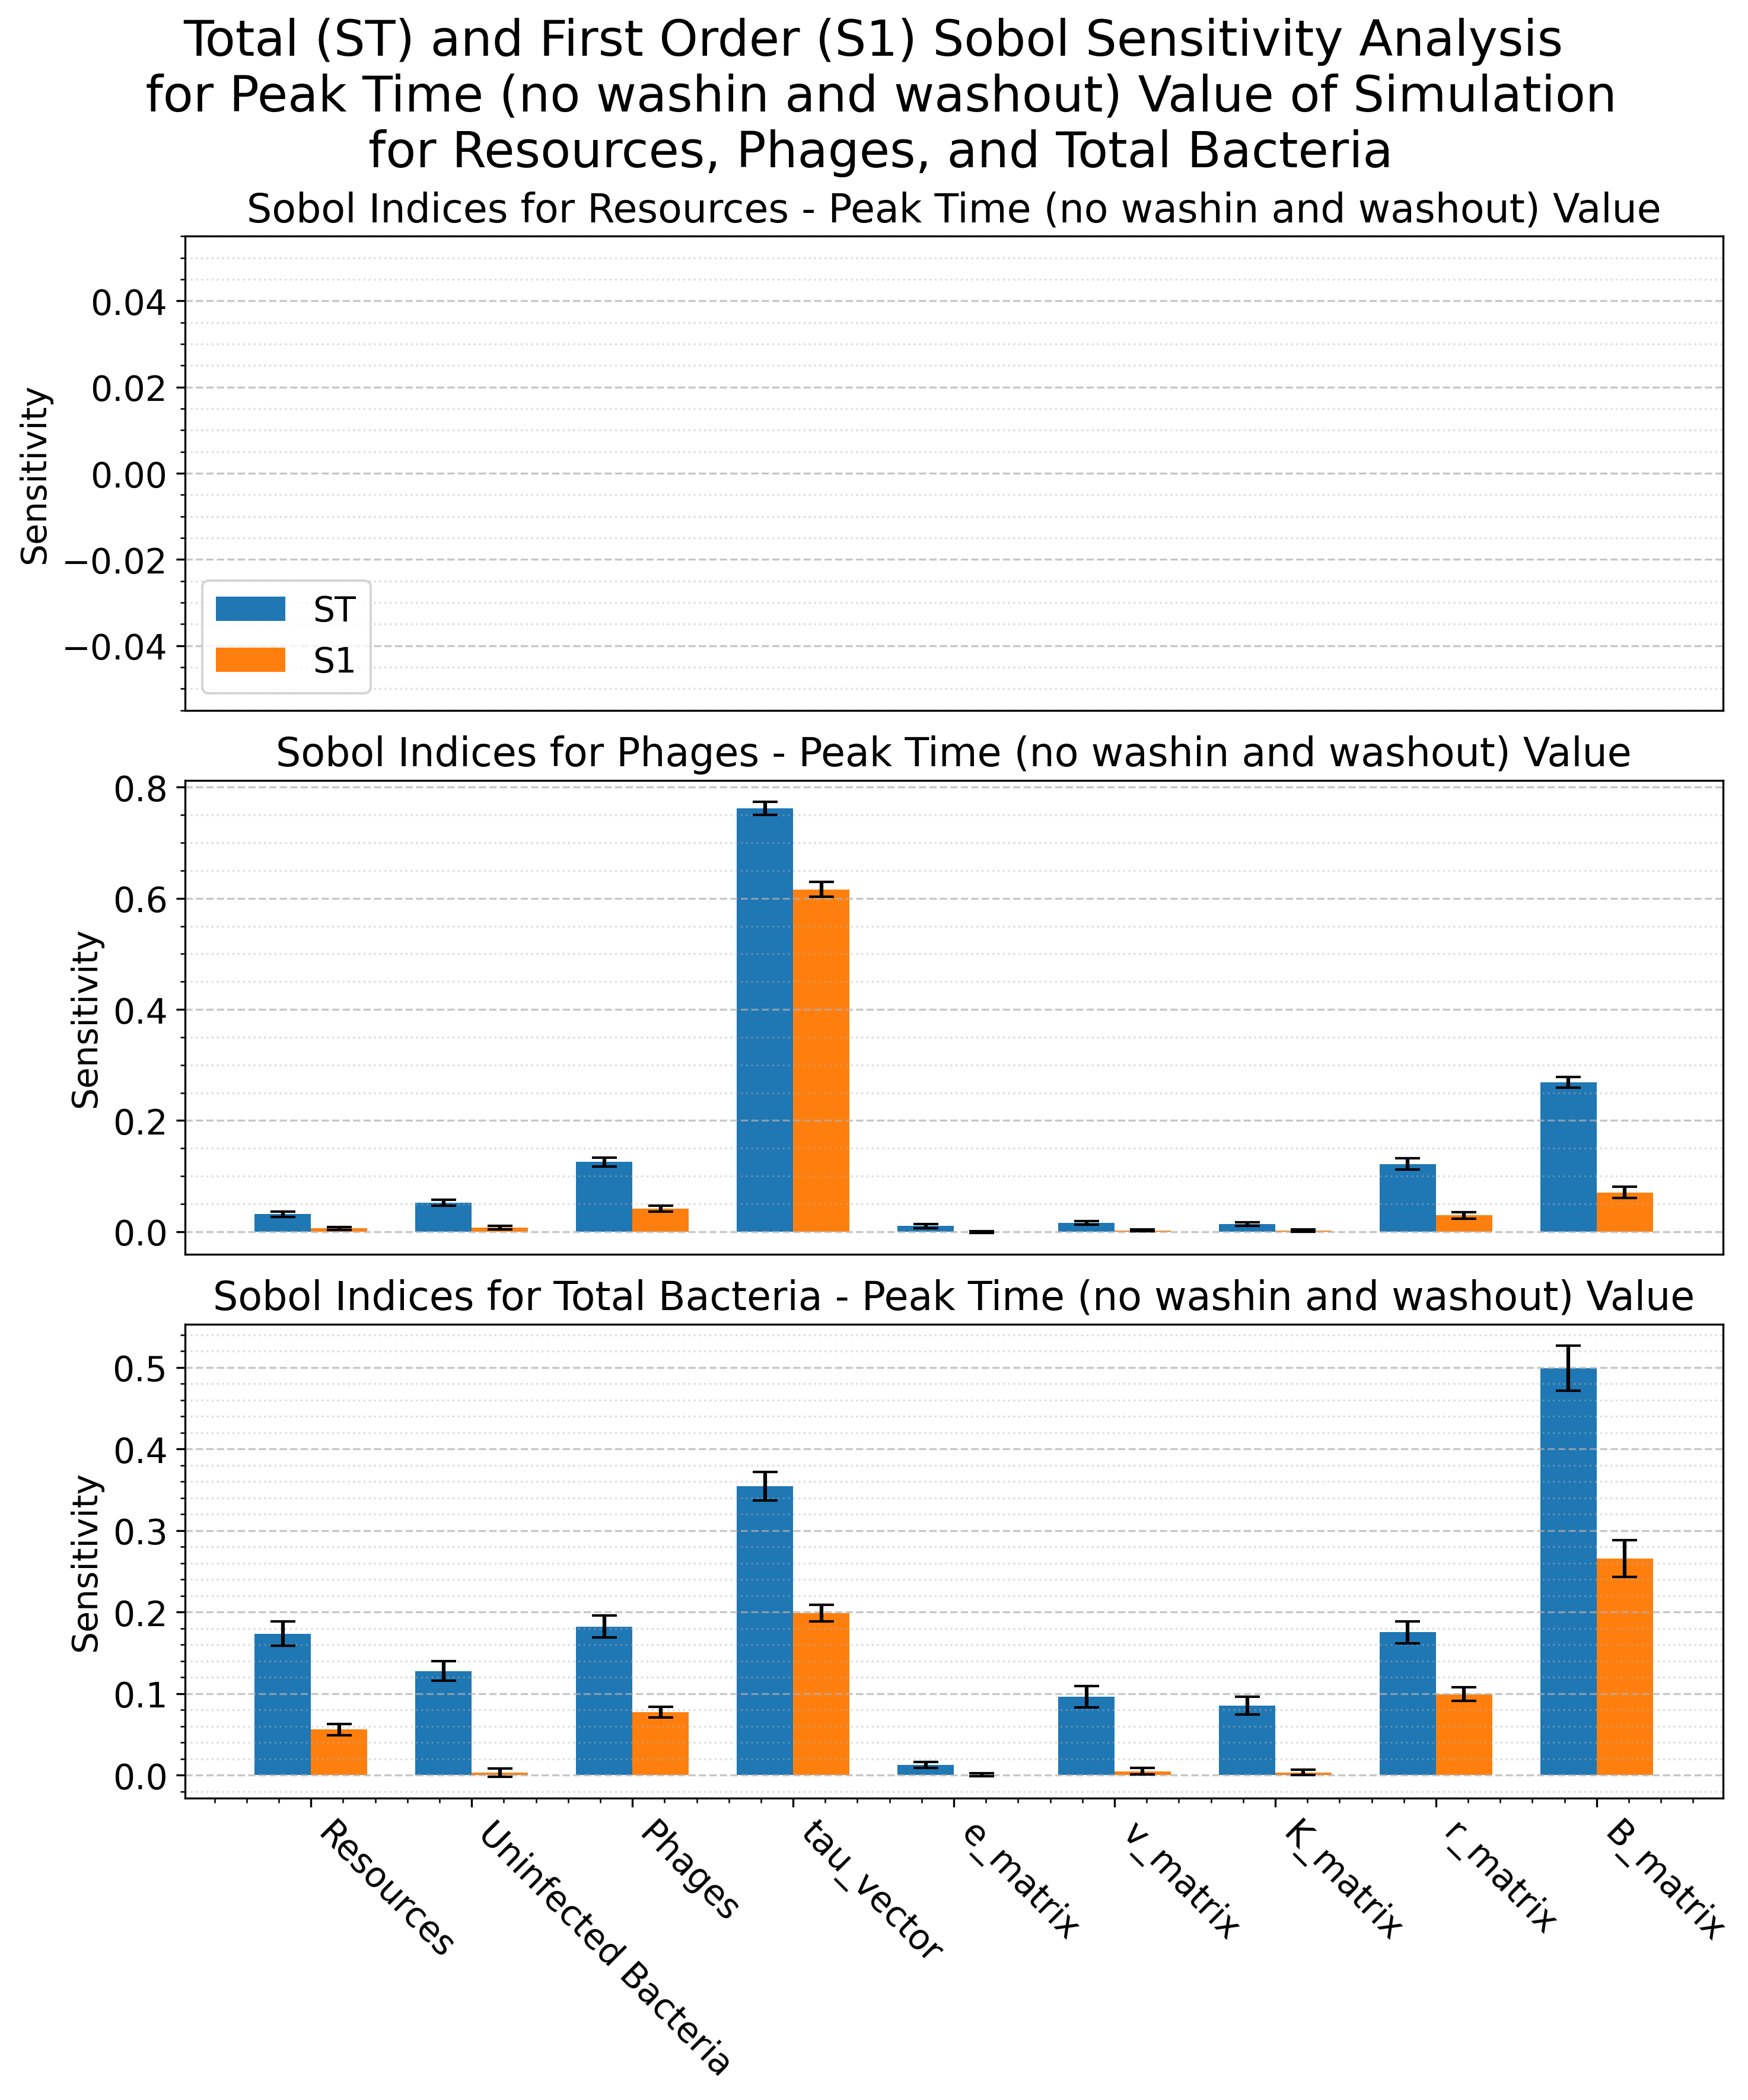
\includegraphics[width=\linewidth]{Plots/Created/SOBOL/SOBOL_analysis_1749708738_Peak_Time_(no_washin_and_washout).png}
        \caption{
            Time of peak value, no washin and washout. 
        }
        \label{fig:created:Sobol_peak_time_no_wi_wo}
    \end{subfigure}
    \caption{
        Sobol analyses for the final, peak, and time of peak value, without a washin and washout rate.
        The input value ranges to test each parameter used for this Sobol test can be found in \Cref{tab:appendixE:Sobol_analysis_values}, except washin and washout is 0. 
    }
    \label{fig:created:Sobol_no_wi_wo}
\end{figure}

\section{Graph Behavior with IVA}
Knowing how a change in parameter values across a wide range of values affects the curve is important. 
The sections below quantitatively and qualitatively elaborate how a change in parameter value across multiple values changes the shape of the population curves. 
Only the most important parameters identified in the Sobol section, along with the initial resource, uninfected bacteria, and phage value will be analyzed. 
So initial resource, uninfected bacteria, phage, $\tau$, $r$, and $\beta$ will be analyzed. 
The default parameter values can be found in \Cref{tab:appendixE:a_good_curve}, but are given in the text as well. 
The sections below use an IVA run to analyze the change in behavior across a wide range of values. 
Each figure from which the conclusions are made can be found in \Cref{sec:apendixF:graph_behavior_with_IVA}. 
$\omega^i$ and $\omega^o$ are not included despite having a large impact as seen in \Cref{sec:AppendixF:sobol_analysis_with_washin_and_washout} because $\omega^i$ and $\omega^o$ are not a part of the original Golding model. 

\subsection{$R$}
The initial resource concentration values were tested across a range from 1 resource to 500 resources, with a default value of 200 resources. 
The IVA run and results can be found at \Cref{fig:created:IVA_IVAtable_resource}. 
All resource values are depleted at around the same time, within 1 time unit of each other. 
As the resource concentration increases, the time it takes for the uninfected bacteria to peak goes from 0.5 time units to 4.12 time units. 
The infected bacteria face the opposite, where it as the resource concentration increases, the time to peak goes from 9.5 time units to 4.9 time units. 
The same behavior is exhibited for the phages, except the time goes from 14 time units to 6.3 time units. 
The phage population showed a huge variety in max population, ranging from a max of 464 phages to 17,200 phages, a 37x difference. 
The max bacteria sum population varied from 55 to 3106 total bacteria, a difference of 56.5 times. \Cref{fig:created:IVA_IVAtable_resource}. 

\subsection{$U$}
The initial uninfected bacteria population values were tested across a range from 1 uninfected bacteria to 100 uninfected bacteria, with a default value of 200 uninfected bacteria. 
The IVA run and results can be found at \Cref{fig:created:IVA_IVAtable_uninfected_bacteria}. 
As the initial uninfected bacteria population increases, the resources are consumed faster, the bacteria populations grow faster and peak earlier. The phages were able to grow faster. The phages peaked at 5.7 time units for 100 initial uninfected bacteria, while for small initial uninfected, the phages peaked at 10.3 time units. Varying the uninfected bacteria had little influence on the max value reached. There is a difference of 600 phages between the phages that started with 1 uninfected and 100 uninfected bacteria. The difference in total bacteria peak values is 173. Changing the uninfected bacteria had little influence on the peak values, but had a large influence on the time of peak value. \\

\subsection{$P$}
The initial phage population values were tested across a range from 1 phage to 50 phages, with a default value of 10 phages. 
The IVA run and results can be found at \Cref{fig:created:IVA_IVAtable_phages}. 
The differing phages values had almost no influence on resource consumption, and limited impact on the peak value and time to peak value for the bacteria and phages. 
The difference between the peak and time of peak values is minor. 
The final phage population at $t=15$ was 9436 for an initial phage value of 50, while for an initial phage value of 1, the final phage value reached 10,676. 
The time of peak difference is just 1.44 time units. 
As the phage value increases, the time for the uninfected, infected, and phages to reach their peak decreases in time. 

\subsection{$\tau$}
The $\tau$ parameter values were tested across a range from 0.5 to 3.5, with a default parameter value of 0.7. 
The IVA run and results can be found at \Cref{fig:created:IVA_IVAtable_tau}. 
$\tau$ has no influence on how fast the resources are being consumed. 
But as $\tau$ increased, the time for the infected bacteria population to peak went from 4.43 to 11.21 time units, and the time it took for the phages to peak went from 5.49 to 14.70 time units, a 2.53 times and 2.68 times increase in time length. 
Smaller $\tau$ values resulted in larger final phage populations and smaller total bacteria populations. 
The peak value and time of peak value for varying $\tau$ values shows little difference for the bacteria sum, ranging from a peak of 1,444 to 1,702 total bacteria and time of peak of 3.74 to 3.82 time units, a difference of 0.08 time units. 
As $\tau$ increases, the infection process will take longer, and it will take longer for the bacteria to die. 
Dying later means the phage's population experiences a delay in growth, taking longer to grow and peak in population value. 
More bacteria can grow in the meantime, and consume resources. 
The bacteria will take longer to peak as there is less initial pressure from the phages. 

\subsection{$r$}
The $r$ parameter values were tested across a range from 0.001 to 0.2, with a default parameter value of 0.001. 
The IVA run and results can be found at \Cref{fig:created:IVA_IVAtable_r}. 
For small $r$ values, all resources are consumed by $t=5$, while for large $r$ values only 13.12 resources were consumed as not enough bacteria were created throughout the simulation to consume all the resources. 
As $r$ increases, the time to reach the max value decreases for the uninfected and infected bacteria, and phages. The delay in phage value went from 6.32 to 2.35 time units, and the total bacteria went from 3.81 to 0.59 time units. 
However, for large $r$ values, there was little phage and bacteria growth. 
For large $r$ values, there was a max of 154 phages and 79 bacteria, while for small $r$ values there was a peak of 10,464 phages and 1,588 total bacteria. 
As $r$ increases, the probability of a successful infection increases, increasing the adsorption rate of phages and causing the phages to grow and peak earlier. 
This higher adsorption rate causes the bacteria to be infected faster, causing them to die faster. 
Lower $r$ values gives more time for the bacteria to grow, which gives the phages more bacteria to infect, leading to higher final phage populations at the end.

\subsection{$\beta$}
The $\beta$ parameter values were tested across a range from 1 to 100, with a default parameter value of 10. 
The IVA run and results can be found at \Cref{fig:created:IVA_IVAtable_beta}. 
For large $\beta$ values, not every resource was consumed, similar to large $r$ values, where for $\beta=100$, 89 resources were consumed. 
As $\beta$ increases, the time to peak for the infected bacteria and phages temporarily increases before decreasing. 
For the uninfected bacteria, the time to peak (does not change for $\beta=1$ to $\beta=10$) takes 3.8 time units, but for larger $\beta$ values, the time to peak decreases to a minimum of 1.94 time units. 
There was a large difference in phage population values, ranging from 4.54 final phages to 42,570 phages, a 9,376 times increase in phage value. 
As $\beta$ increases in value, more phages are being created upon lysis, which infects the bacteria. 
For $\beta$ less than 10, the bacteria growth is restricted by latency, how fast a bacterium can go through the infection process, while for $\beta$ greater than 10 the system changes to an adsorption limited regime, where the phages can't adsorb to the bacteria fast enough, allowing bacteria to grow faster and peak earlier. 
As more phages are being produced, more bacteria are being infected, so the bacteria population starts to die out earlier, with fewer bacteria being produced. 
With fewer bacteria, fewer resources are being consumed. 

\section{Initial Value Analysis Results}
\label{sec:results:initial_value_analysis}
\Cref{fig:created:initial_value_analysis_UB_50_500_a_good_plot_2} and \Cref{fig:created:initial_value_analysis_UB_50_500_a_good_plot} illustrate how varying the initial uninfected bacteria population from 1 to 500 (using 100 different starting values) affects the dynamics and time of peak population of phage and total bacteria populations using the 95\% rule. 

\Cref{fig:created:initial_value_analysis_UB_50_500_a_good_plot_2} perfectly replicates Figure 1 (\Cref{fig:sourced:Mulla}) of \citet{mullaExtremeDiversityPhage2024}. 
As the initial bacteria population increases, the time to reach the phage and bacteria sum peak decreases, following $y = -0.8648\cdot ln(x) + 9.7911$ and $y = -1.0056\cdot ln(x)+7.7626$, with $R^2=0.9800, 0.9988$ respectively. 

\Cref{fig:created:initial_value_analysis_UB_50_500_a_good_plot} on the other hand shows different behavior. 
As the initial bacteria population decreases from 500 to 100, \Cref{fig:created:initial_value_analysis_UB_50_500_a_good_plot_2} exhibits the same behavior. 
There is a change in behavior at 100 and less initial uninfected bacteria. 
Instead of following the predicted line like in \Cref{fig:created:initial_value_analysis_UB_50_500_a_good_plot_2}, the curve for the phages decrease non-monotonically.
The bacteria plateau before starting to increase again. 

The fitted linear regression curves follow $y = -0.1292\cdot ln(x) + 10.1462$ and $y = -0.6234\cdot ln(x)+6.9602$, with $R^2=0.5406, 0.9206$ respectively. 
The slope tells us how well the uninfected bacteria has an influence on the time of peak value. 
The larger (positive or negative) the slope is, the more impact the uninfected bacteria had on the time of peak value. 
The closer the $R^2$ value is to 1, the more proportion of the variance for the time to peak value is explained by the uninfected bacteria. 
The linear regression curve can not explain the change in limiting regions. 
So for the first curve, the uninfected bacteria had a small influence on the time of peak value, while with the second curve, changing the uninfected bacteria had a larger impact on the time of peak and is considerably more important in explaining the time of peak value. 

\begin{figure}
    \centering
    \begin{subfigure}{1\linewidth}
        \centering
        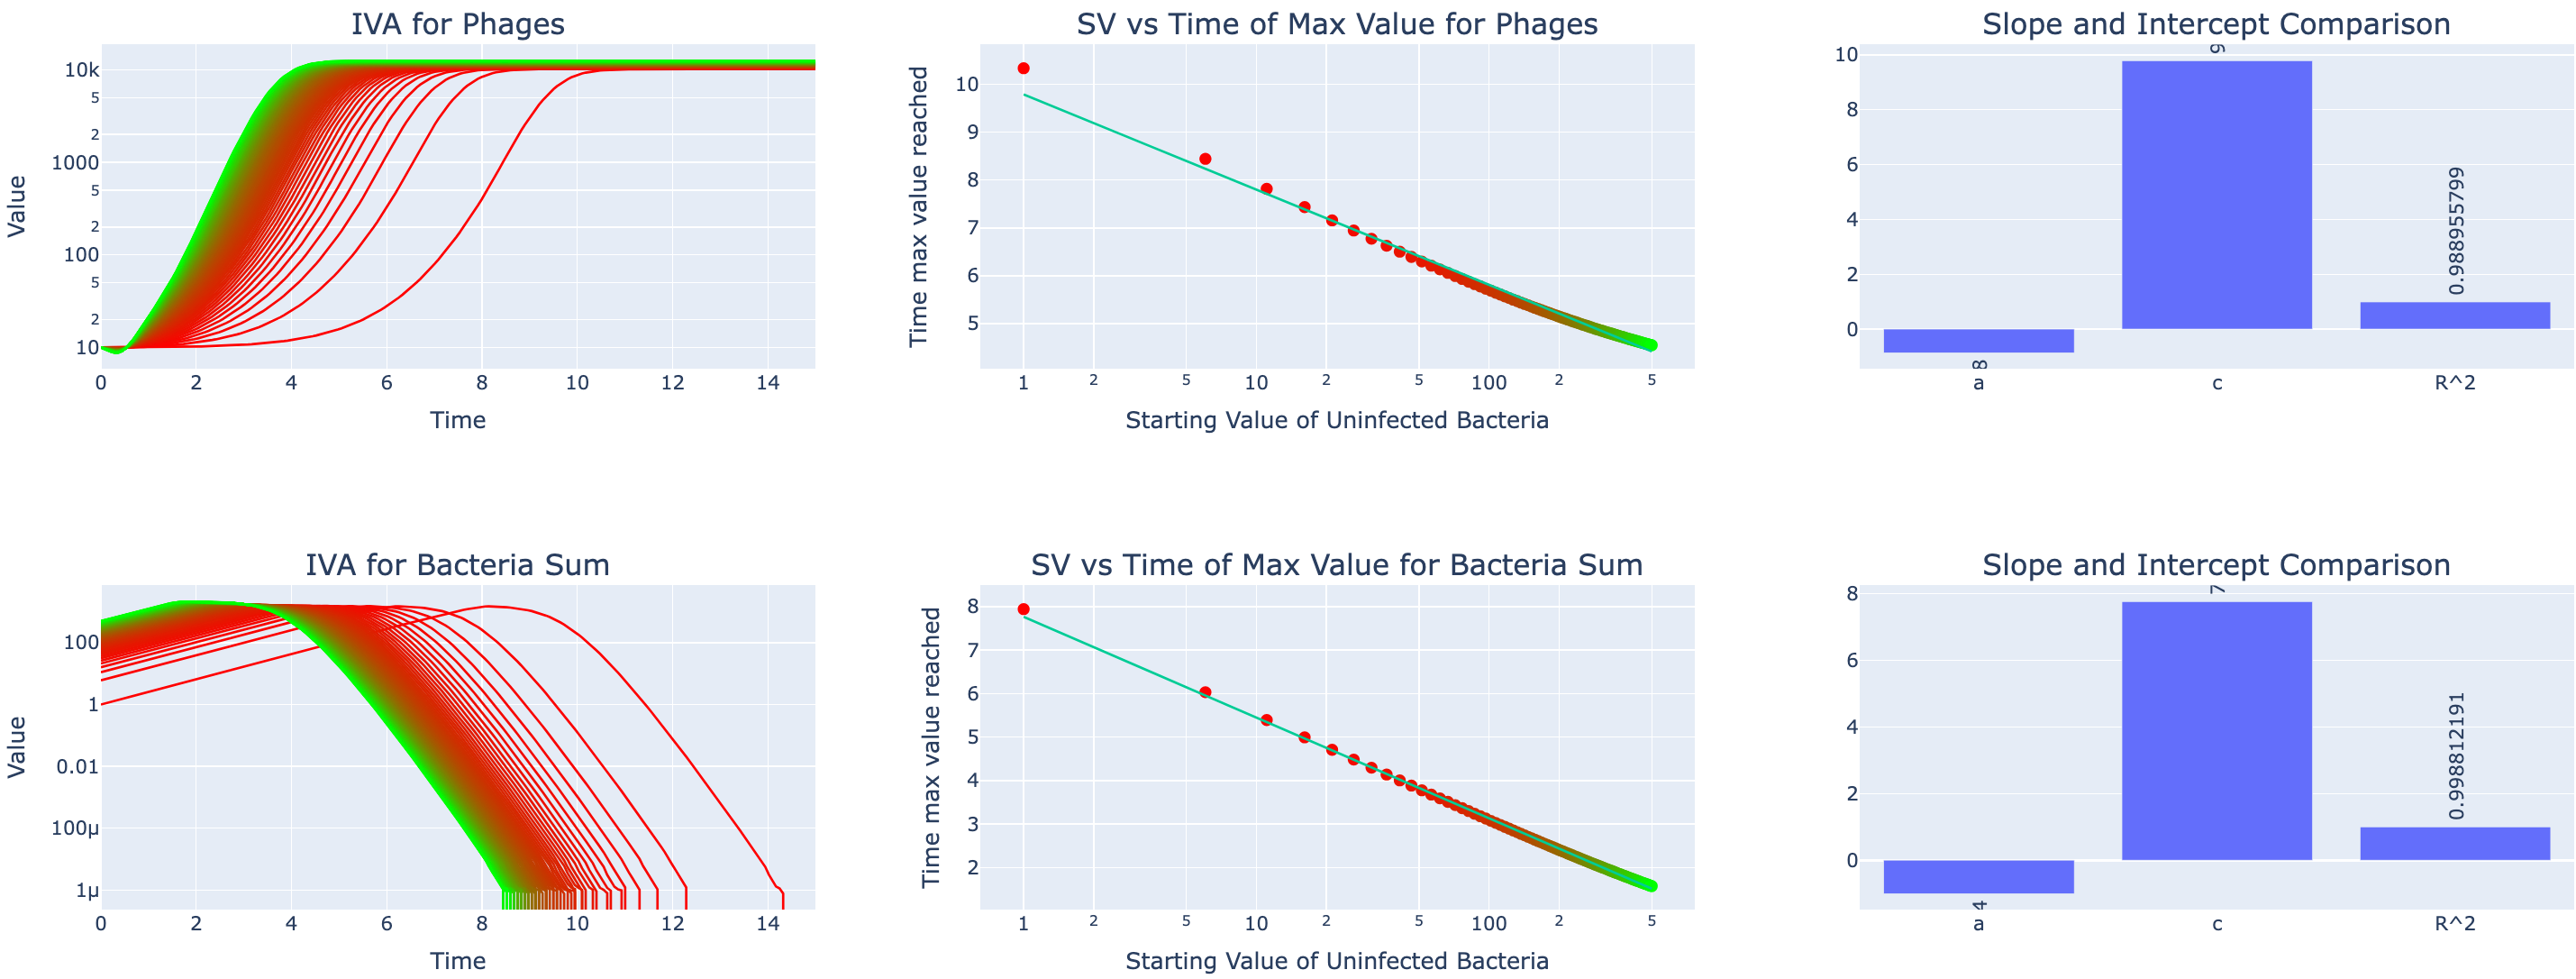
\includegraphics[width=\linewidth]{Plots/Created/IVA/initial_value_analysis_UB_50_500_a_good_plot_2.png}
        \caption{
            IVA for \Cref{tab:appendixE:a_good_curve_2}. 
            Replicates Figure 1 of \citet{mullaExtremeDiversityPhage2024}. 
            The system is adsorption limited \cite{mullaExtremeDiversityPhage2024}. 
        }
        \label{fig:created:initial_value_analysis_UB_50_500_a_good_plot_2}
    \end{subfigure}
    \hfill
    \begin{subfigure}{1\linewidth}
        \centering
        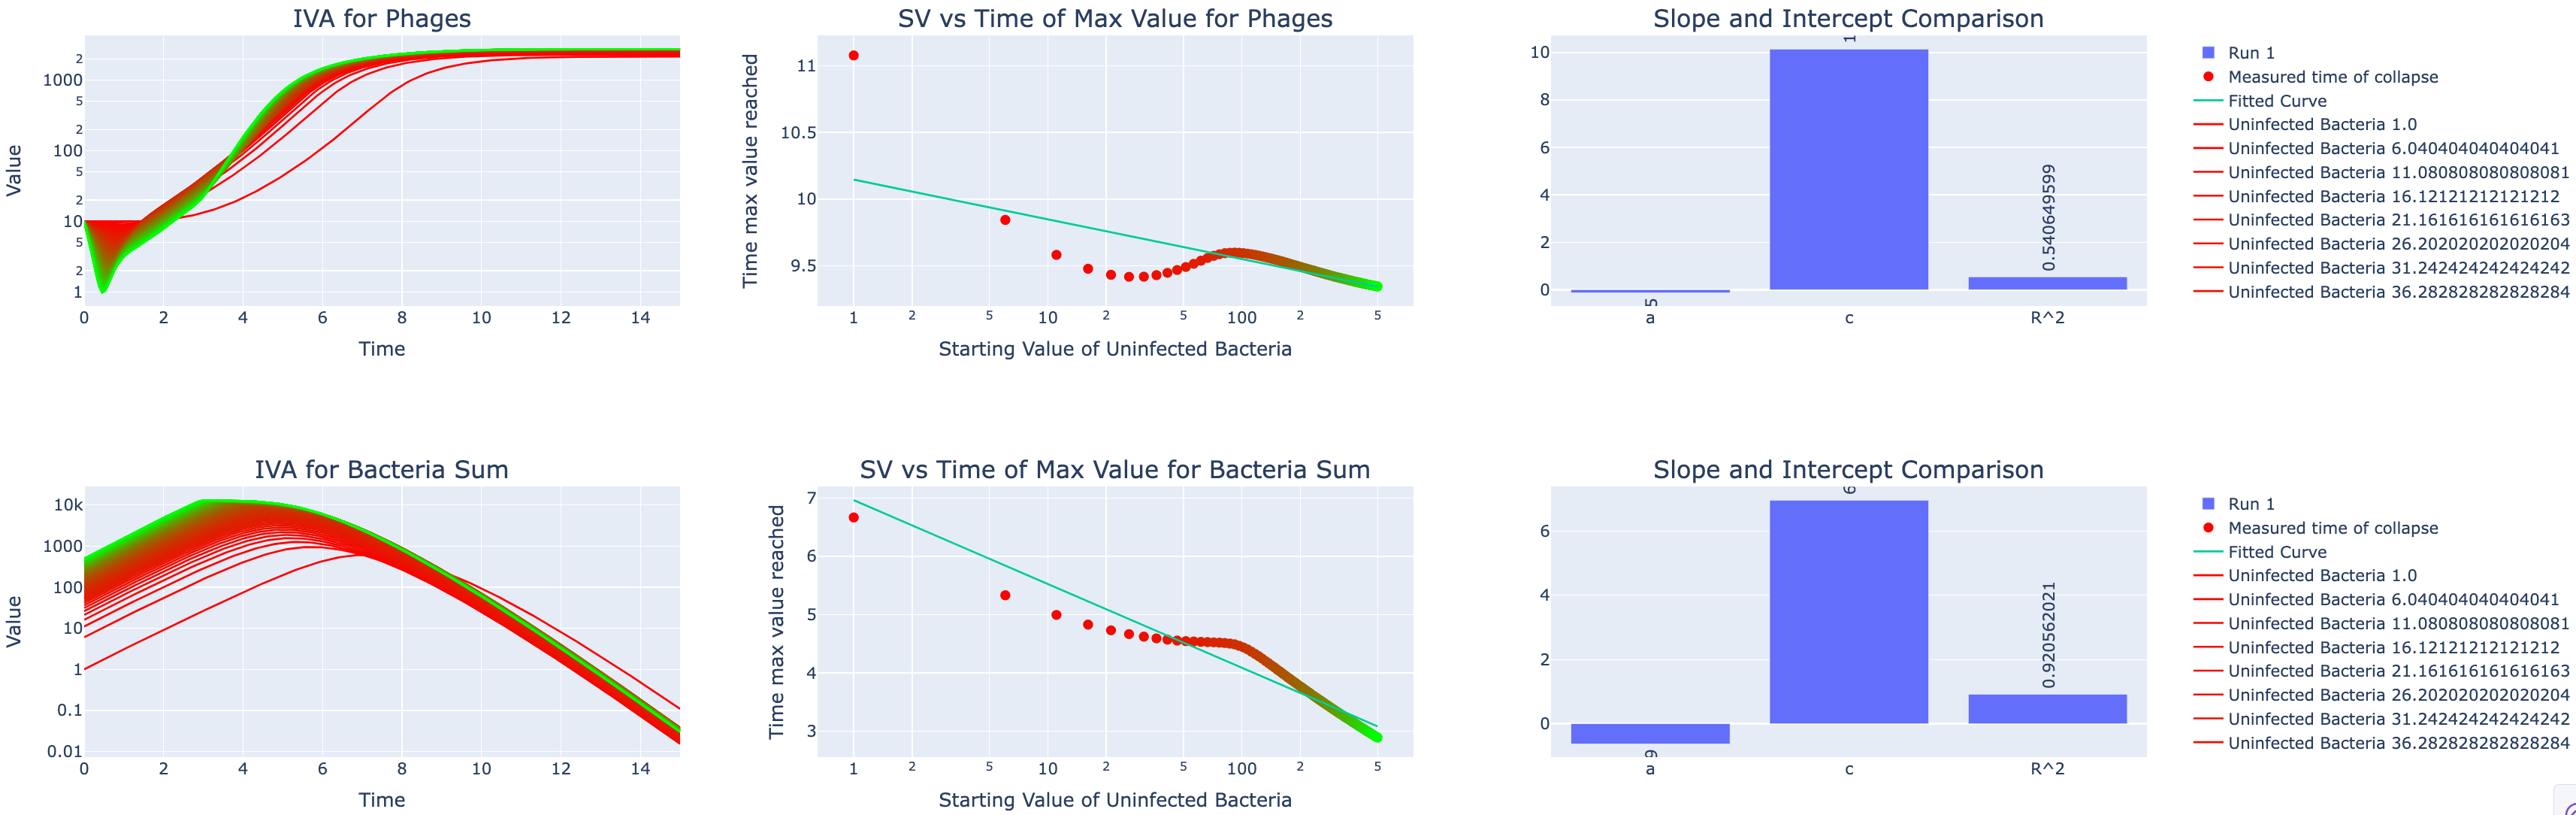
\includegraphics[width=\linewidth]{Plots/Created/IVA/initial_value_analysis_UB_50_500_a_good_plot.png}
        \caption{
            IVA for \Cref{tab:appendixE:a_good_curve}. 
            For uninfected bacteria less than 100, the phage-bacteria interaction is resource limited. 
        }
        \label{fig:created:initial_value_analysis_UB_50_500_a_good_plot}
    \end{subfigure}
    \caption{
        Varying the initial uninfected bacteria concentration, from 50 to 500, with 30 unique values tested. 
        Varying the default parameter values a can have a large influence on how changing the initial bacteria concentration influences the dynamics of the system. 
        The default values for Figure a) and b) can be found at \Cref{tab:appendixE:a_good_curve} and \Cref{tab:appendixE:a_good_curve_2}. 
    }
\end{figure}

\section{Phage Proliferation}
Understanding how phage behavior varies under different conditions, is important. 
Phages have to survive throughout the whole experiment. 
Phages can experience random deactivations or if the replication process is not fast enough, be removed from the system from the washout. 
\label{sec:results:phase_portrait}
\subsection{Phase Portrait}
\Cref{fig:created:phase_portrait_resources_245-265_phages_25-26} shows a phase portrait varying the initial resource and phage concentration. 
The same initial phage values have the same color for the line. 
For phages that start above 25.98, the phage population can proliferate until the washout would eventually remove the phages. 
For phage populations that start below 25.98, the washout removes the phages before the phages had time to infect and kill the bacteria. 
Both regions of phages exhibit consistent behavior, of either going to 0 or proliferating. 
If the phage population started at exactly 25.98, if the initial resources was 260 or above, the phages died out. 
If the initial resource value was 255 or below, the phages proliferated. 

\subsection{An Initial Phage and Resource Analysis for Phage Proliferation}
\Cref{fig:created:phase_portrait_resources_phage} expands on the phase portrait by simulating more values and coloring the square depending on if the phages proliferated or not. 
The initial resource values span from 1 to 500, and the initial phage values range from 25.5 to 26.5, each with 100 unique values sampled.

\Cref{fig:created:phase_portrait_resource_phage_proliferate} zooms into the range $(1-40, 24.2-25)$ for a high detailed view of the behavior happening around initial resources of 10. 
From 1 to around 7 initial resources, fewer phages are needed to ensure proliferation. 
At 7 initial resources, there is a minimum in the phage proliferation boundary. 
From 7 initial resources and upwards, as more resources are added to the system, more phages are needed to ensure proliferation. 
Despite this, the change is tiny, a difference of about 2 phages. 
Considering the range of possible initial phage populations, the phage proliferation boundary is essentially flat. 
Under these parameter values, choosing an initial phage population of 27 or higher will ensure phage proliferation. 
The higher the initial resource concentration, the more final phages will appear. 
As there are more resources, more bacteria can grow from the resources, which in turn allows more phages to grow. 

If there is a higher washout, similar behavior is observed where the phage proliferation boundary exhibits a similar shape to that of \Cref{fig:created:phase_portrait_resources_phage}, except more phages are needed to proliferate. 
If $K$ is increased to a larger value, the minimum in the proliferation boundary is shifted to the right. 

\begin{figure}[]
    \centering
    \begin{subfigure}{0.49\linewidth}
        \centering
        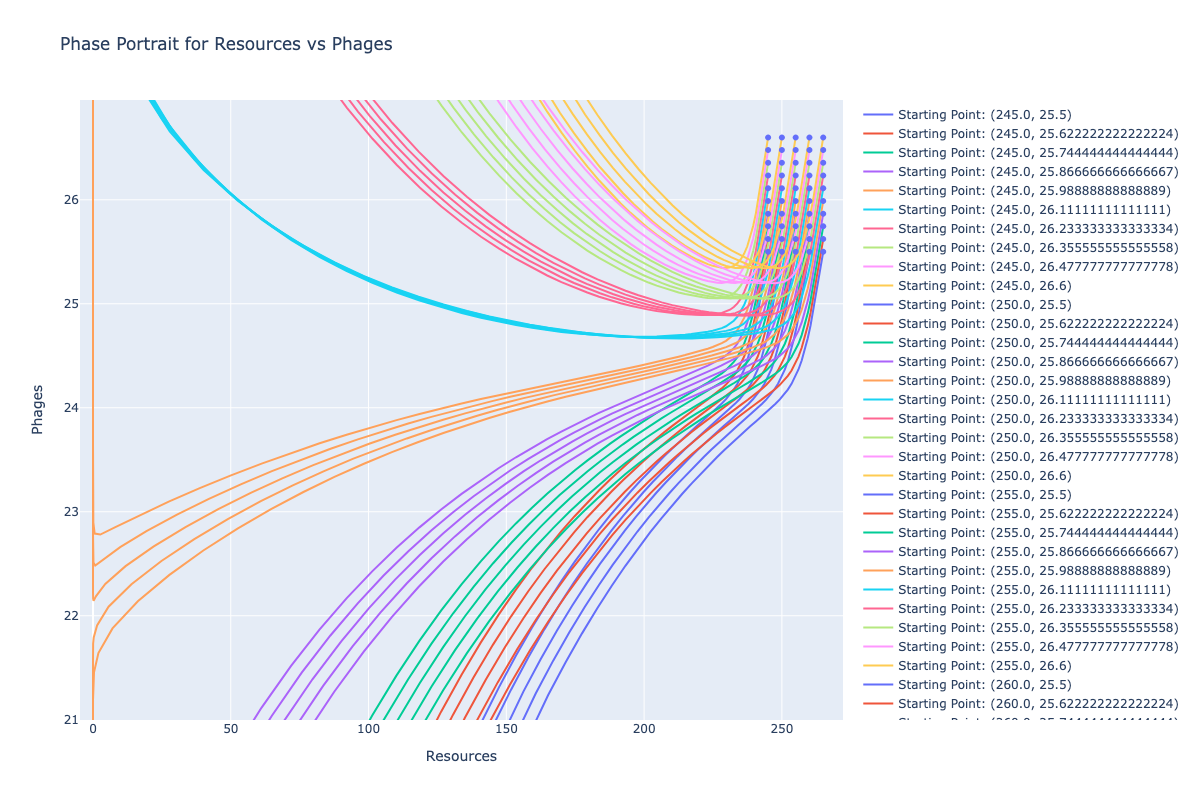
\includegraphics[width=1\textwidth]{Plots/Created/PP/phase_portrait_resources_245-265_phages_25-26.png}
        \caption{
            Zoomed in plot of a phase portrait with varying resource and phage population from 245-265 and 25.5-26.5 respectively. 
            Each row has its own line color. 
            Diverging behavior can be seen for the orange line (phage=25.98). 
        }
        \label{fig:created:phase_portrait_resources_245-265_phages_25-26}
    \end{subfigure}
    \hfill
    \begin{subfigure}{0.49\linewidth}
        \centering
        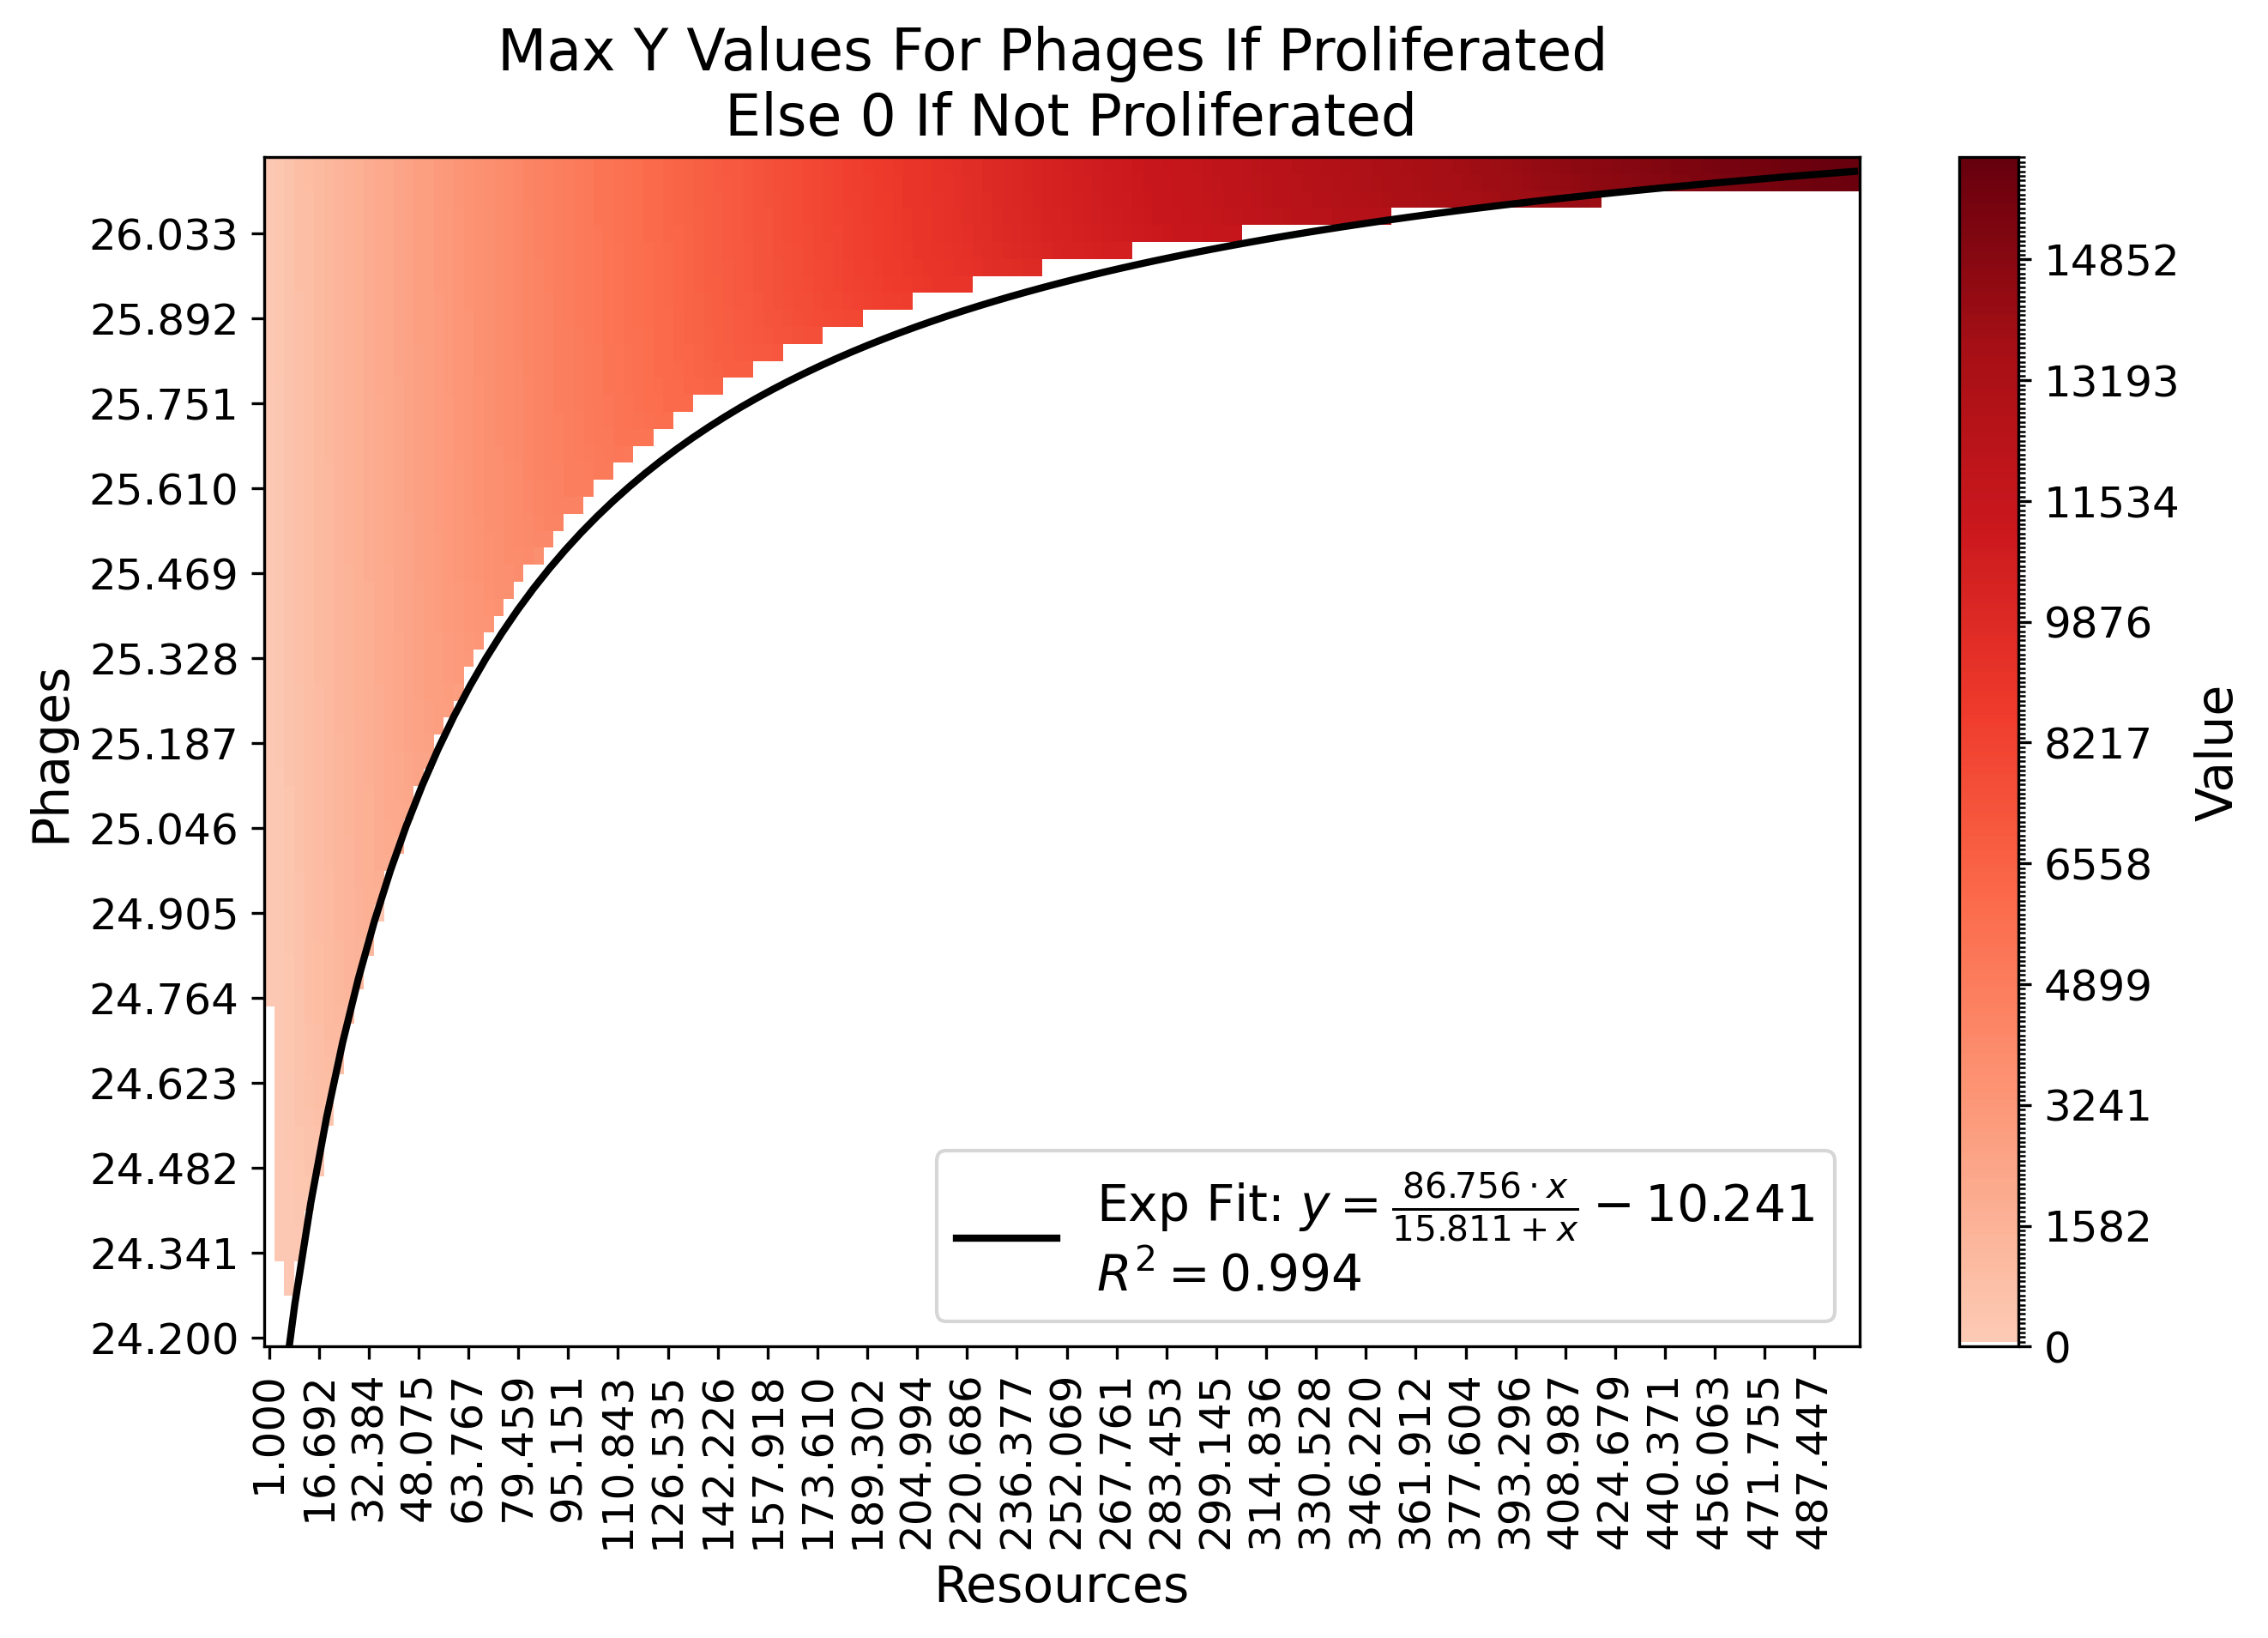
\includegraphics[width=\linewidth]{Plots/Created/PP/phase_portrait_resources_phage.png}
        \caption{
            Phage population proliferation as a function of initial resource and phage concentrations. 
            While the color appears uniform along the vertical axis, each cell is actually a slightly different value. 
            The phage-resource proliferation boundary follows a fitted Monod equation.
        }
        \label{fig:created:phase_portrait_resources_phage}
    \end{subfigure}
    \hfill
    \begin{subfigure}{0.49\linewidth}
        \centering
        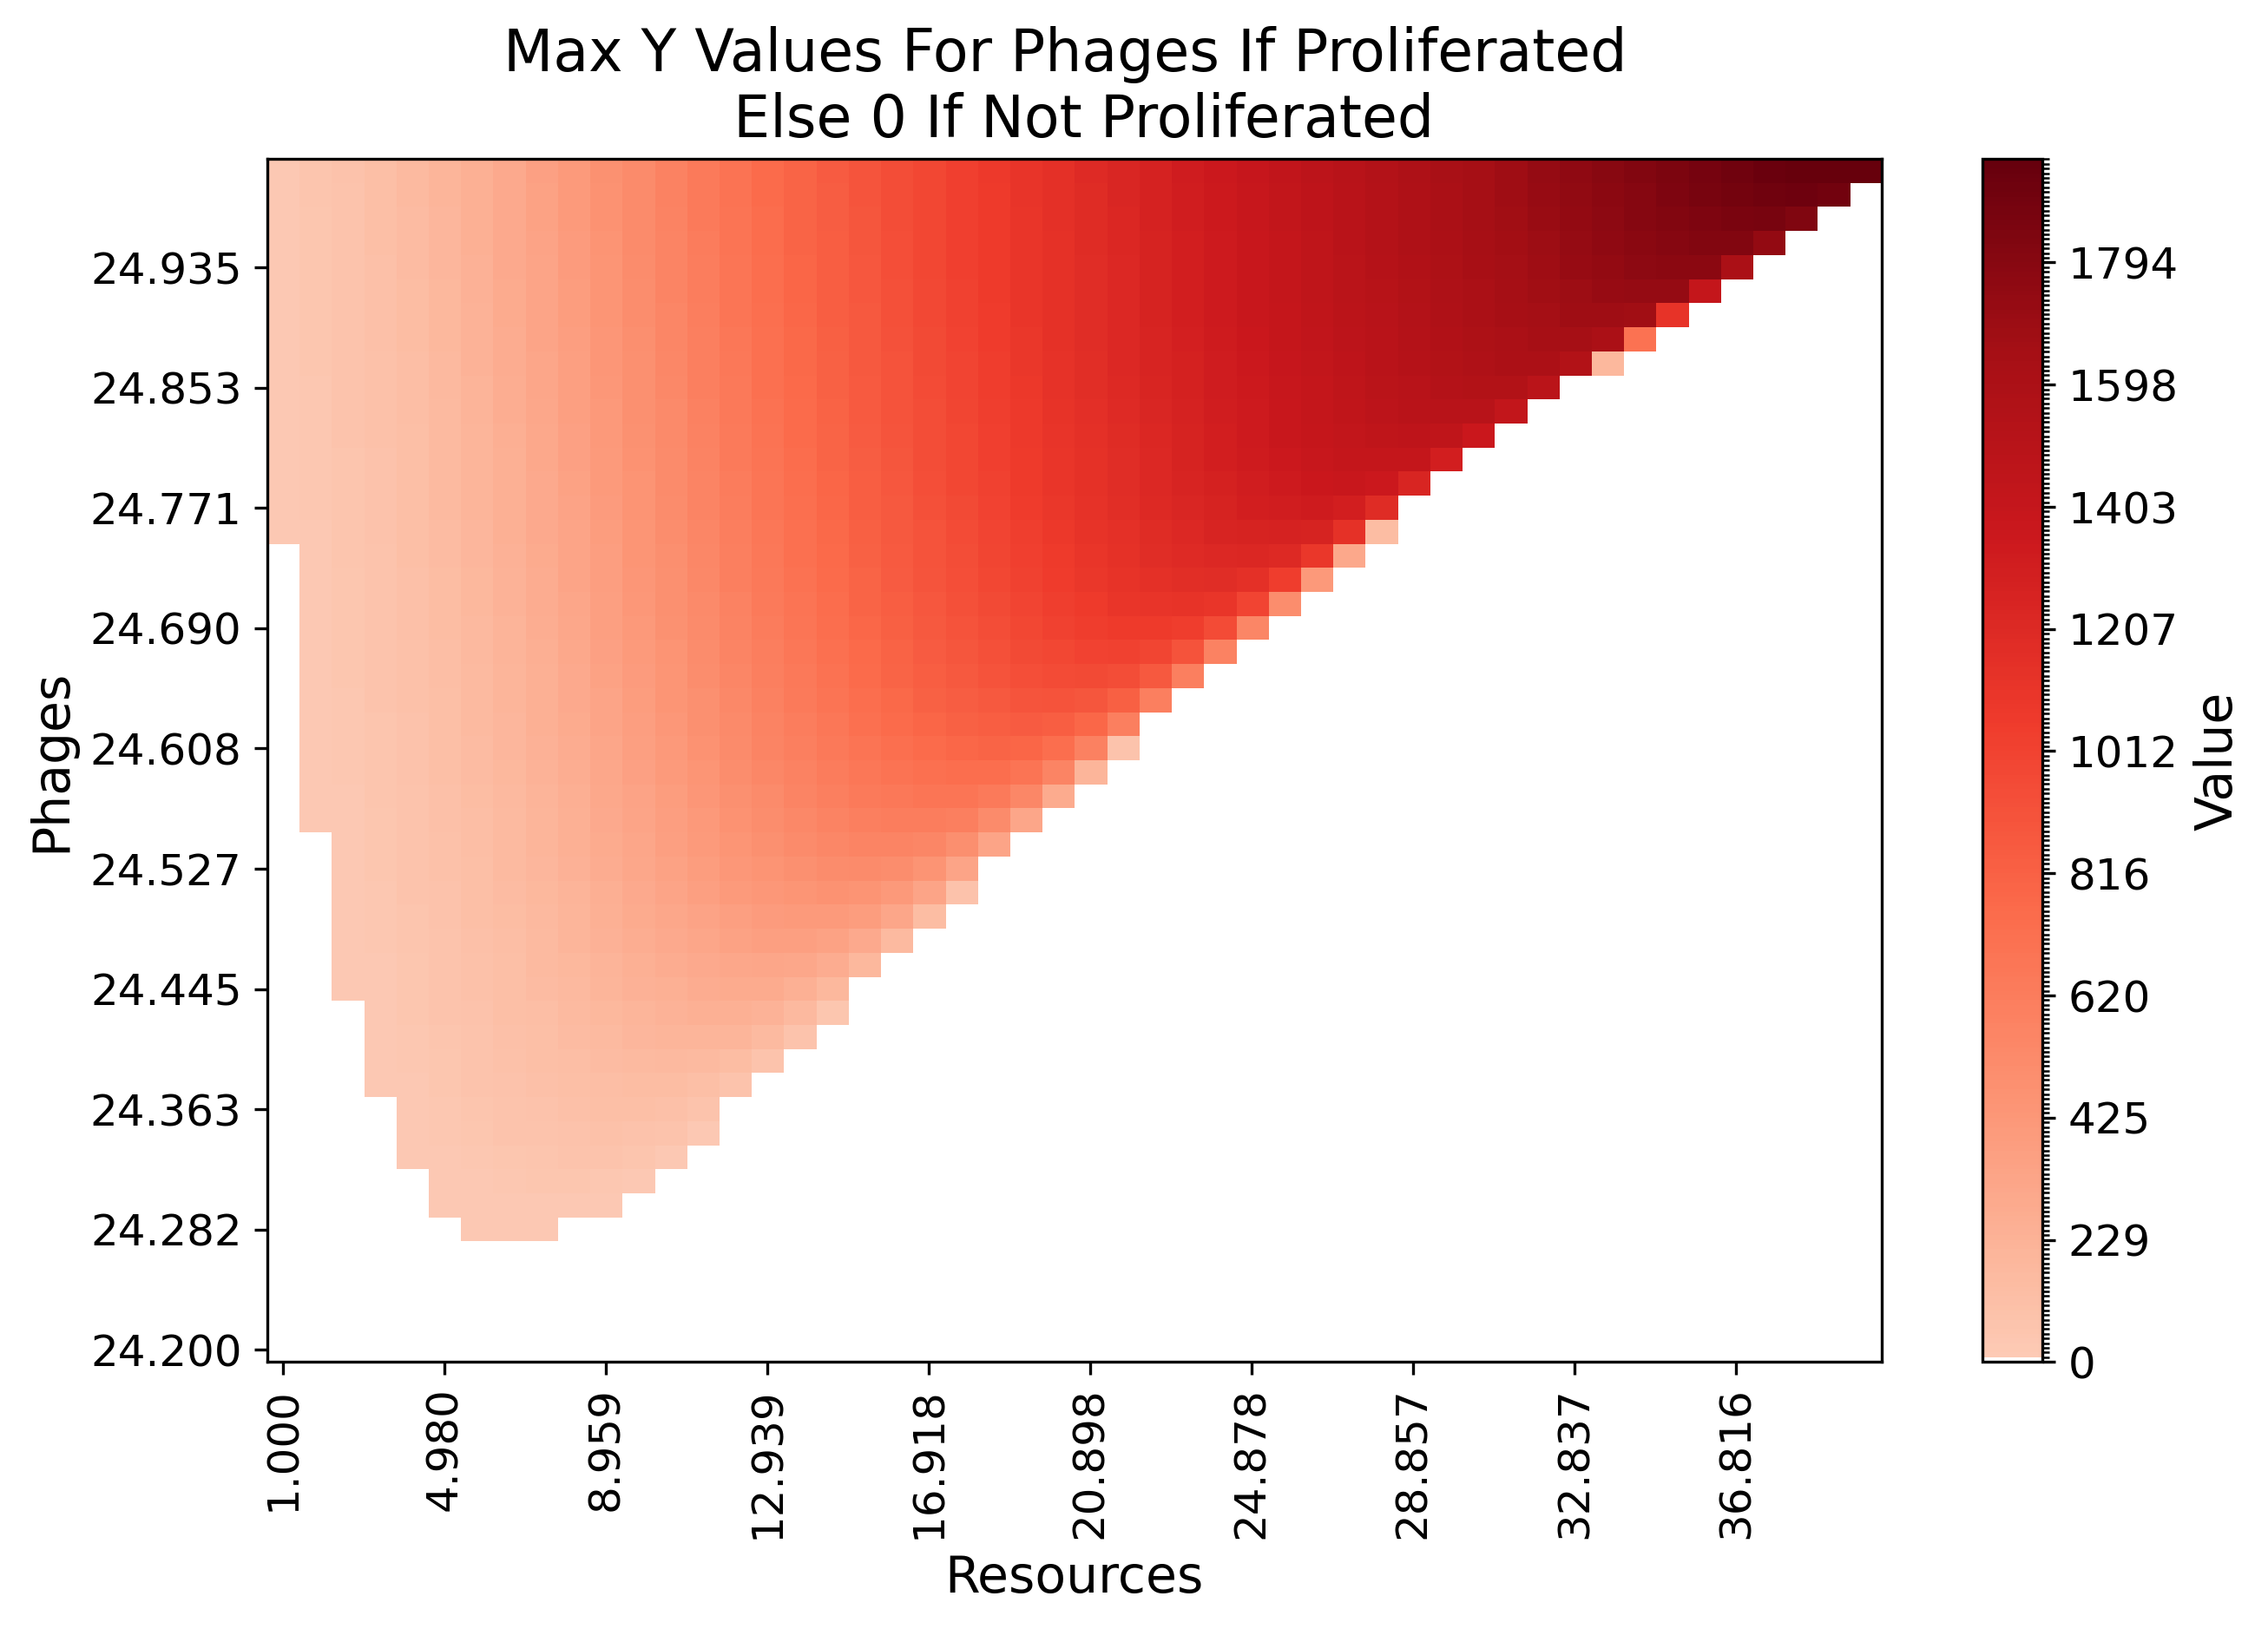
\includegraphics[width=\linewidth]{Plots/Created/PP/phase_portrait_resources_phage_2.png}
        \caption{
            Zoomed in to analyze the regime of behavior change near resources$=10$. 
        }
        \label{fig:created:phase_portrait_resources_phage_2}
    \end{subfigure}
    \caption{
        Varying initial resources and initial phages and the resulting proliferation and fitted proliferation curve. 
        The box is colored red if the phages proliferated for that condition, and white if the phages died out. 
        Phages proliferated if they reached 2 times their initial population at any point in time in the simulation. 
        This simulation used the values from \Cref{tab:appendixE:a_good_curve_2}, but with washout set to 0.02 instead of 0. 
    }
    \label{fig:created:phase_portrait_resource_phage_proliferate}
\end{figure}

\subsection{An Initial Phage, Bacteria, and Resource Analysis for Phage Proliferation}
The initial resource concentration had some, but very limited impact on if the initial phage concentration would affect if the phages proliferate. 
Within the context of the basic Golding model, the initial uninfected bacteria population is one of three parameters that a researcher can easily control, with the other two being the initial resource and initial phage. 
For low initial uninfected bacteria populations, it will be harder for the phages to proliferate. 
There is not enough bacteria to infect before the washout will remove the phages from the system. 
While for large initial uninfected bacteria populations it will be easier for the phages to proliferate such that the washout won't immediately wash the phages out. 
So I extend the initial resource and phage population analysis by adding a third dimension to the analysis, the initial uninfected bacteria population. 
The aim of adding the uninfected bacteria is to see how the initial uninfected bacteria will 1) affect if the phage can proliferate, and 2) affect the max population that the phages can reach. 

\Cref{fig:created:3D_phase_portrait} has three axes, the initial phage, resource, and bacteria population value. 
The initial uninfected bacteria did not have a significant impact on the 1) if the phages would proliferate, and 2) by how much the phages would proliferate. 
If spliced along the bacteria axis, there is little difference in the shape of the curve. 
It was expected that as the uninfected bacteria count would increase there would be significantly fewer phages that would be needed to ensure phage proliferation. 
However, there is not a significant change in if the phages proliferated and by how much. 

This suggests that under a washout situation, ensuring that there are enough phages is the most important factor to ensure that the phages are not washed out. 

\begin{figure}[ht!]
    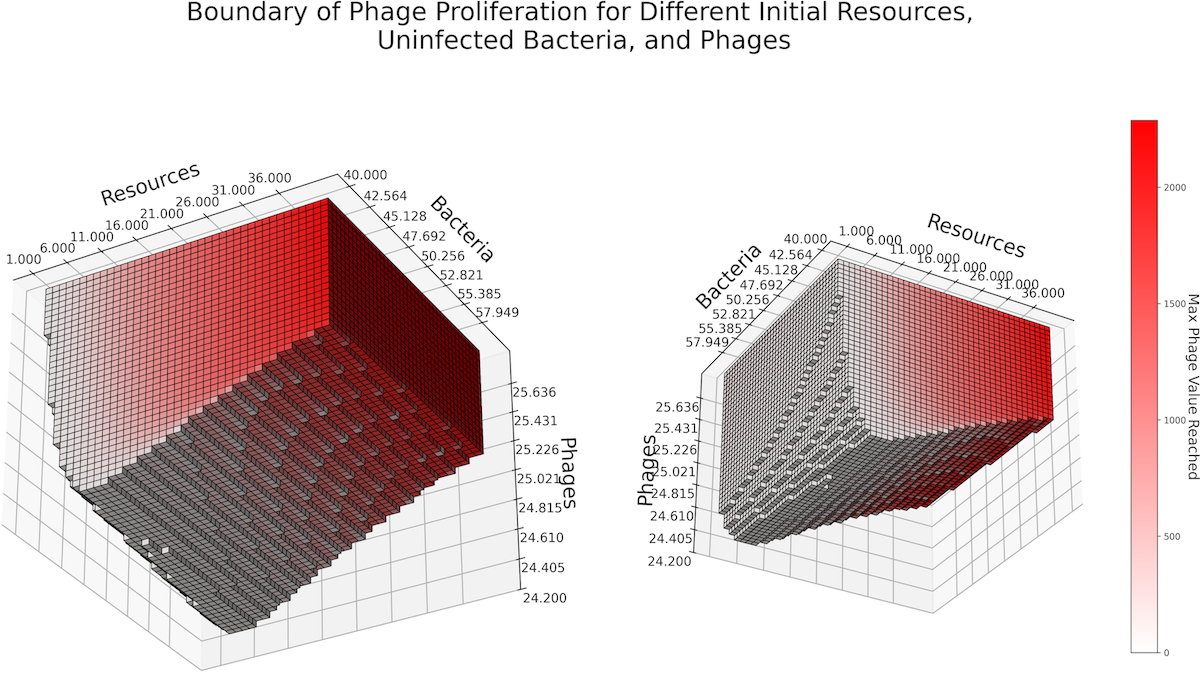
\includegraphics[width=1\textwidth]{Plots/Created/PP/3d_plot_resource_bacteria_phage.png}
    \centering
    \caption{
        3D plot of phage proliferation, dependent on initial resource, uninfected bacteria, and phage population. 
        Color scaling from white to red, color is dependent on the max phage population reached. 
    \label{fig:created:3D_phase_portrait}
    }
\end{figure}

\section{Plotting Parameter Change — $3\times 2\times 3$ Model}
Now that we have identified the most important parameters in the Golding model, we can analyze how the curve shapes change across a range of parameters for a larger model. 
Knowing how multiple parameters influence the output is important. 
As the complexity of the model input increases, interactions, and their parameter values play an important role in determining which phage or bacteria can survive. 
The interactions (or lack thereof) will 

The larger model will exhibit different behavior than a $1\times 1\times 1$ model due to the many interactions. 
The differing parameter values across each interaction will influence how fast each population can grow and die. 
A $3\times 2\times 3$ model was chosen as it is on the boundary between adding more phages, bacteria, or resources would clutter the plot with lines, while still offering behavior that can be compared against one another. 
The graph network that was used can be found at \Cref{fig:ss:example_network}, with the default parameter values found at \Cref{tab:appendixE:complex_model}. 
$B_0$ is infected by $P_1$ and $P_2$, and consumes $R_0$ and $R_1$. 
$B_1$ is infected by $P_0$ and $P_2$, while consuming $R_2$. 


\Cref{fig:created:r_beta_washout_0}, \Cref{fig:created:r_beta_washout_0.02}, and \Cref{fig:created:r_beta_washout_0.05}, show a $7\times7$ matrix of subfigures across washout rates of 0, 0.02, and 0.05
Each subfigure uses a different combination of $r$ and $\beta$ parameter values. 

All initial phage values started at 10. 
This was specifically chosen to show how even though the phage values all start the same, the different parameter values and interactions ultimately influence the population growth. 

If $r$ or $\beta$ is equal to $Original$, then the simulation uses the original parameter values as defined in \Cref{tab:appendixE:complex_model}, otherwise each $r$ and each $\beta$ parameter interaction has the value listed in the subfigure title. 

The columns and rows of each figure show how a change in parameter value affects the curve, while keeping the other parameter the same. 
In $r, \beta, \omega^o=Original, Original, 0$, although not a realistic growth curve, shows how the different parameter values for each interaction uniquely affect the growth rate of each entity, especially the phage population ($P_0$=blue, $P_1$=green, and $P_2$=purple). 
Despite all phages starting at the same population level, within the first two or so time units, $P_1$ has fewer phages than $P_0$ and $P_2$. 
$P_2$ has the fastest initial growth rate, as $P_2$ has the most phages until $t=4$, at which point $P_1$ has a larger phage population. 
$P_2$ reaches its peak population count before $P_0$ or $P_1$, but despite the slower initial growth, $P_0$ and $P_1$ eventually overtake $P_2$ in total phage population. 
$P_2$ also reaches its peak before decreasing in population. 
Since the phage population is reduced by $r_{pb}\cdot(U_b + \sum_{k=1}^M I_{b_k})$, and by specifically choosing the parameter values as used in \Cref{tab:appendixE:complex_model}, behavior that hasn't been seen in a $1\times 1\times 1$ system has been found. 
The complete extinction of the bacteria has been delayed long enough such that at trace amounts, there is phage reduction despite bacteria still existing. 
The peak times for $P_0$, $P_1$, and $P_2$ are $t=6.33, 7.99, 4.52$, a difference of $3.47$ time units. 

Contrast that with the phage population dynamics of that with $r, \beta, \omega^o = Original, 100, 0$, the phage populations do not show notable dynamics. 
The peak times are more similar and consistent to one another ($t=5.50, 7.01, 6.78$, a difference of $1.51$ time units). 
The phage population curve all appear the same, with slightly slower growth rates. 
There is no crossing of phage populations unlike with $r, \beta, \omega^o=Original, Original, 0$. 

The highlighted example demonstrated the dynamics and influence that multiple agents can have on the final output. 

The top row of \Cref{fig:created:r_beta_washout_0.02} shows how the phages and resources died out relative to the top row of \Cref{fig:created:r_beta_washout_0}. 
Even with a high burst value, the phages could not defeat the pressure from the washout. 
But by changing the $r$ value from $r=0.001$ to $r=0.041$, the phages were able to save themselves and proliferate. 

\begin{figure}[]
    \centering
    \begin{subfigure}{0.49\linewidth}
        \centering
        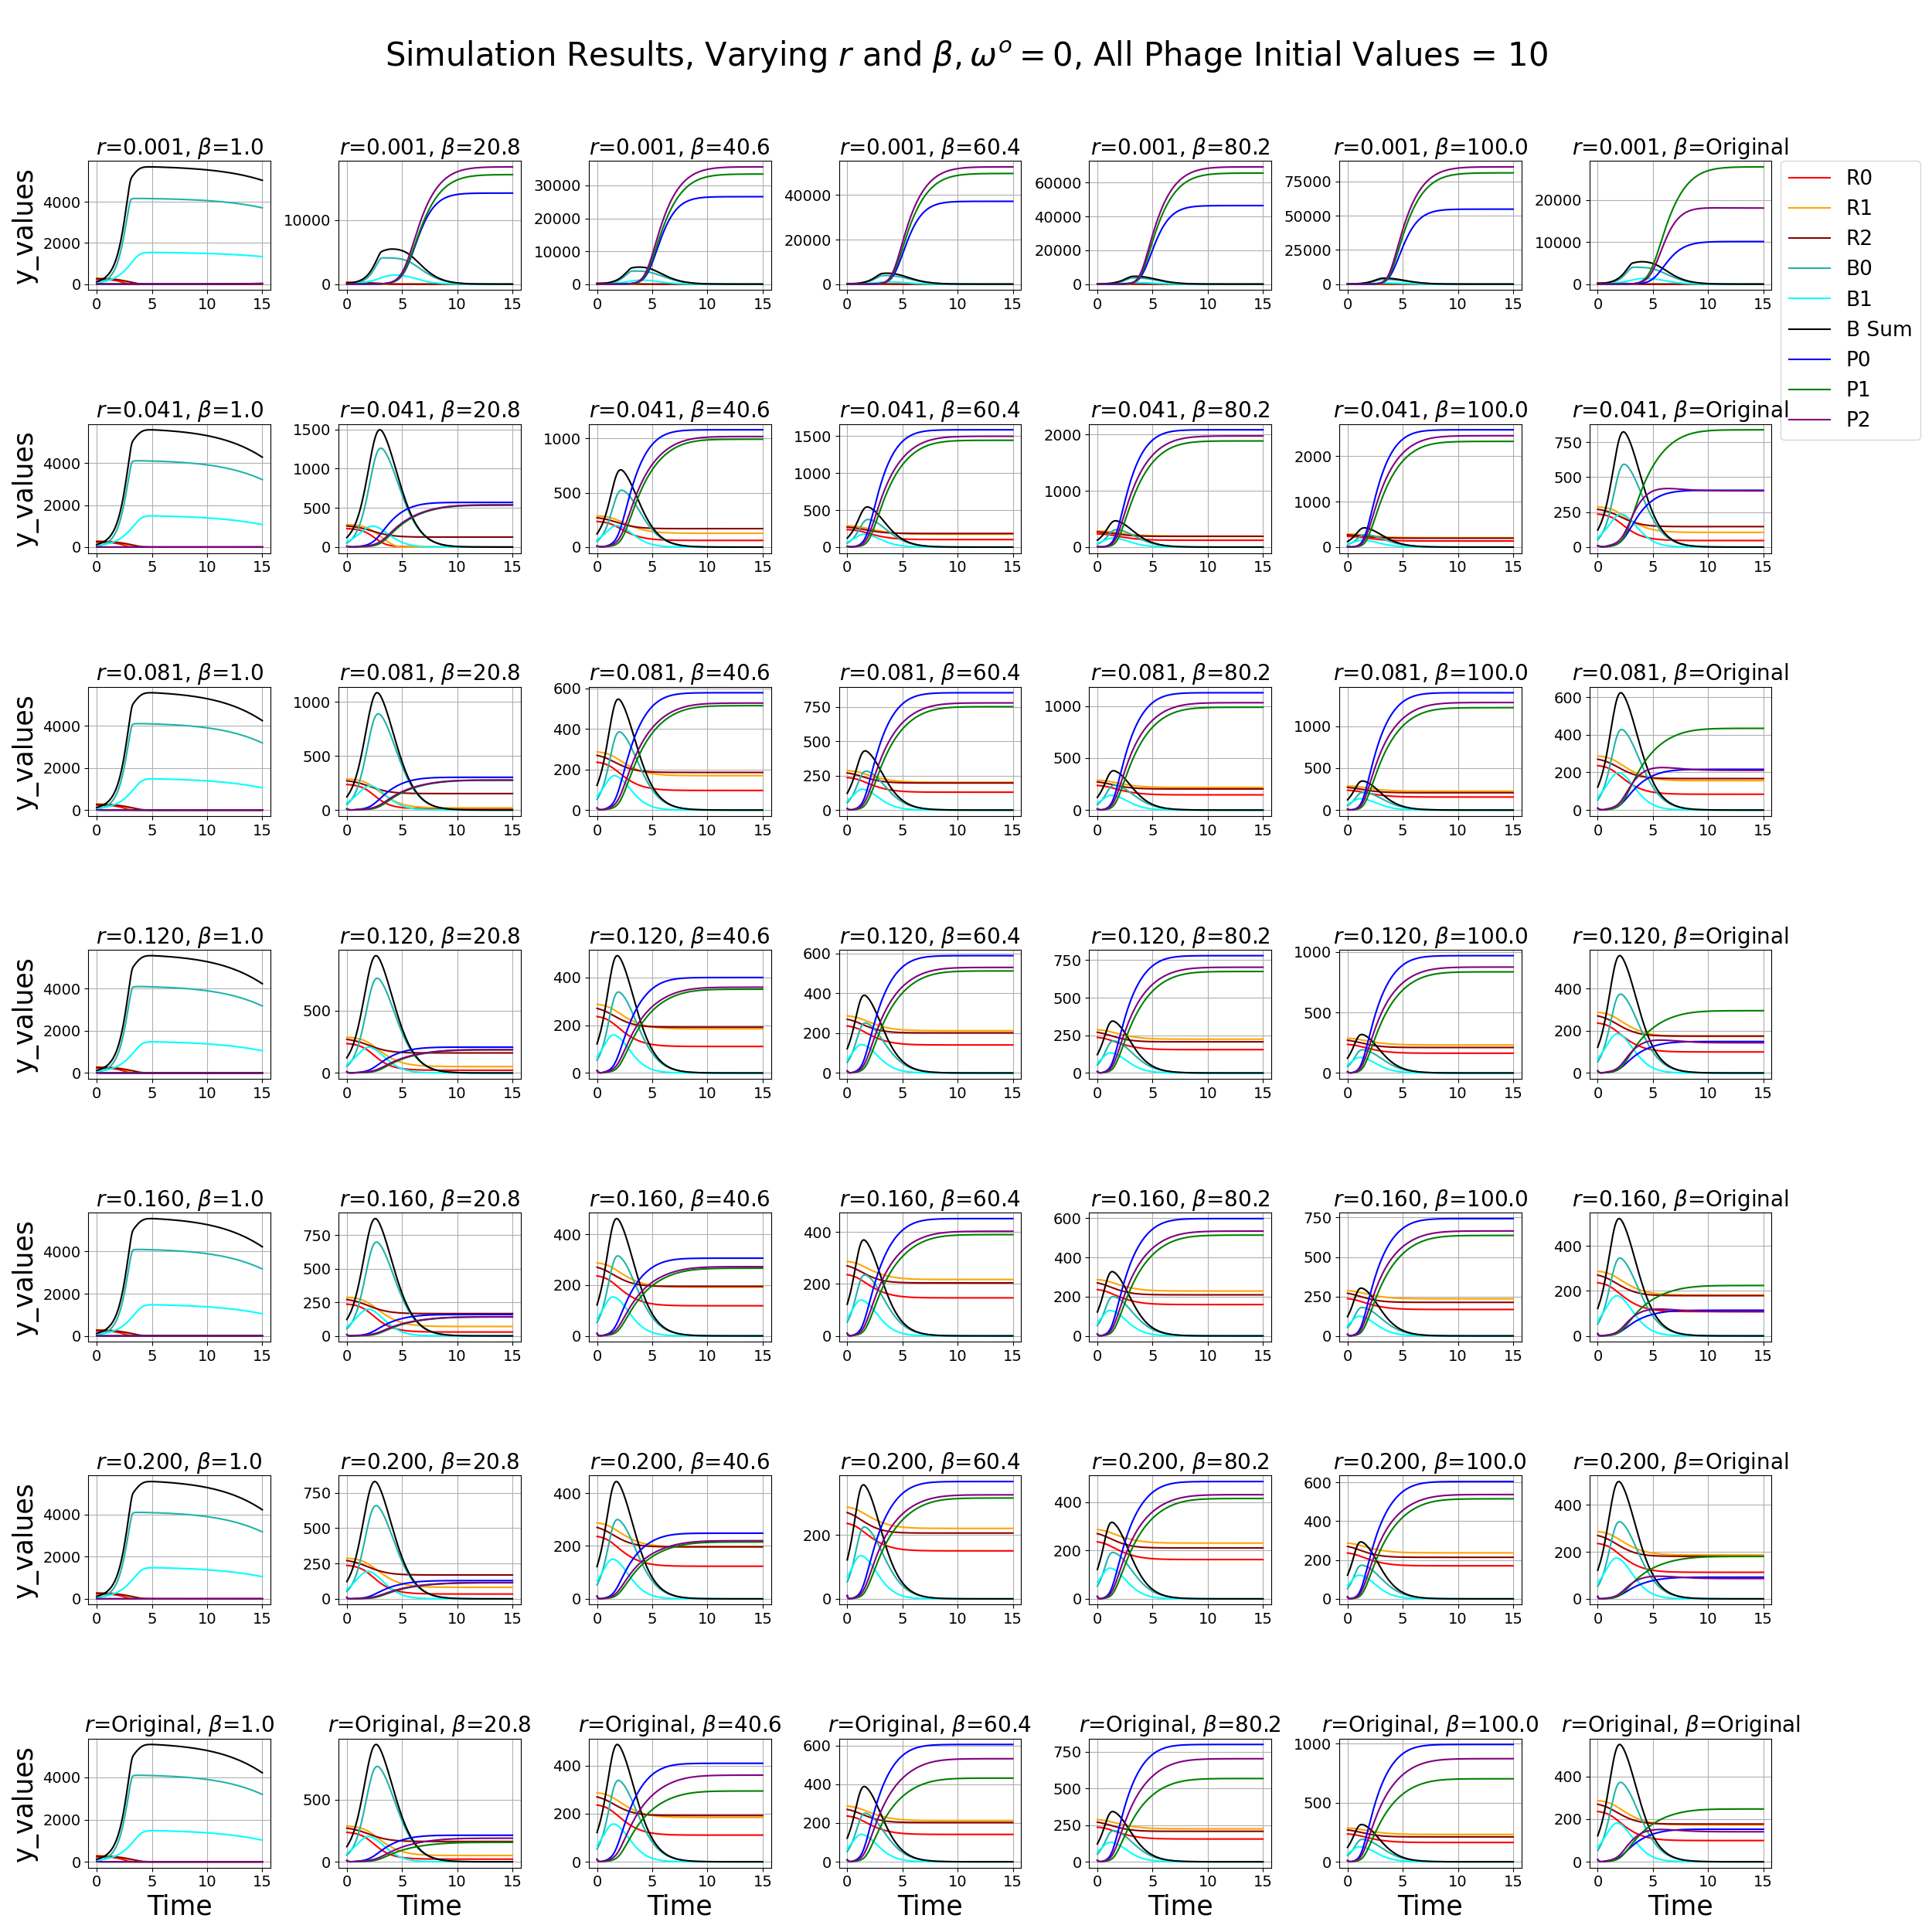
\includegraphics[width=\linewidth]{Plots/Created/UA/r_beta_washout_0.png}
        \caption{
            Washout $\omega^o=0$. 
        }
        \label{fig:created:r_beta_washout_0}
    \end{subfigure}
    \hfill
    \begin{subfigure}{0.49\linewidth}
        \centering
        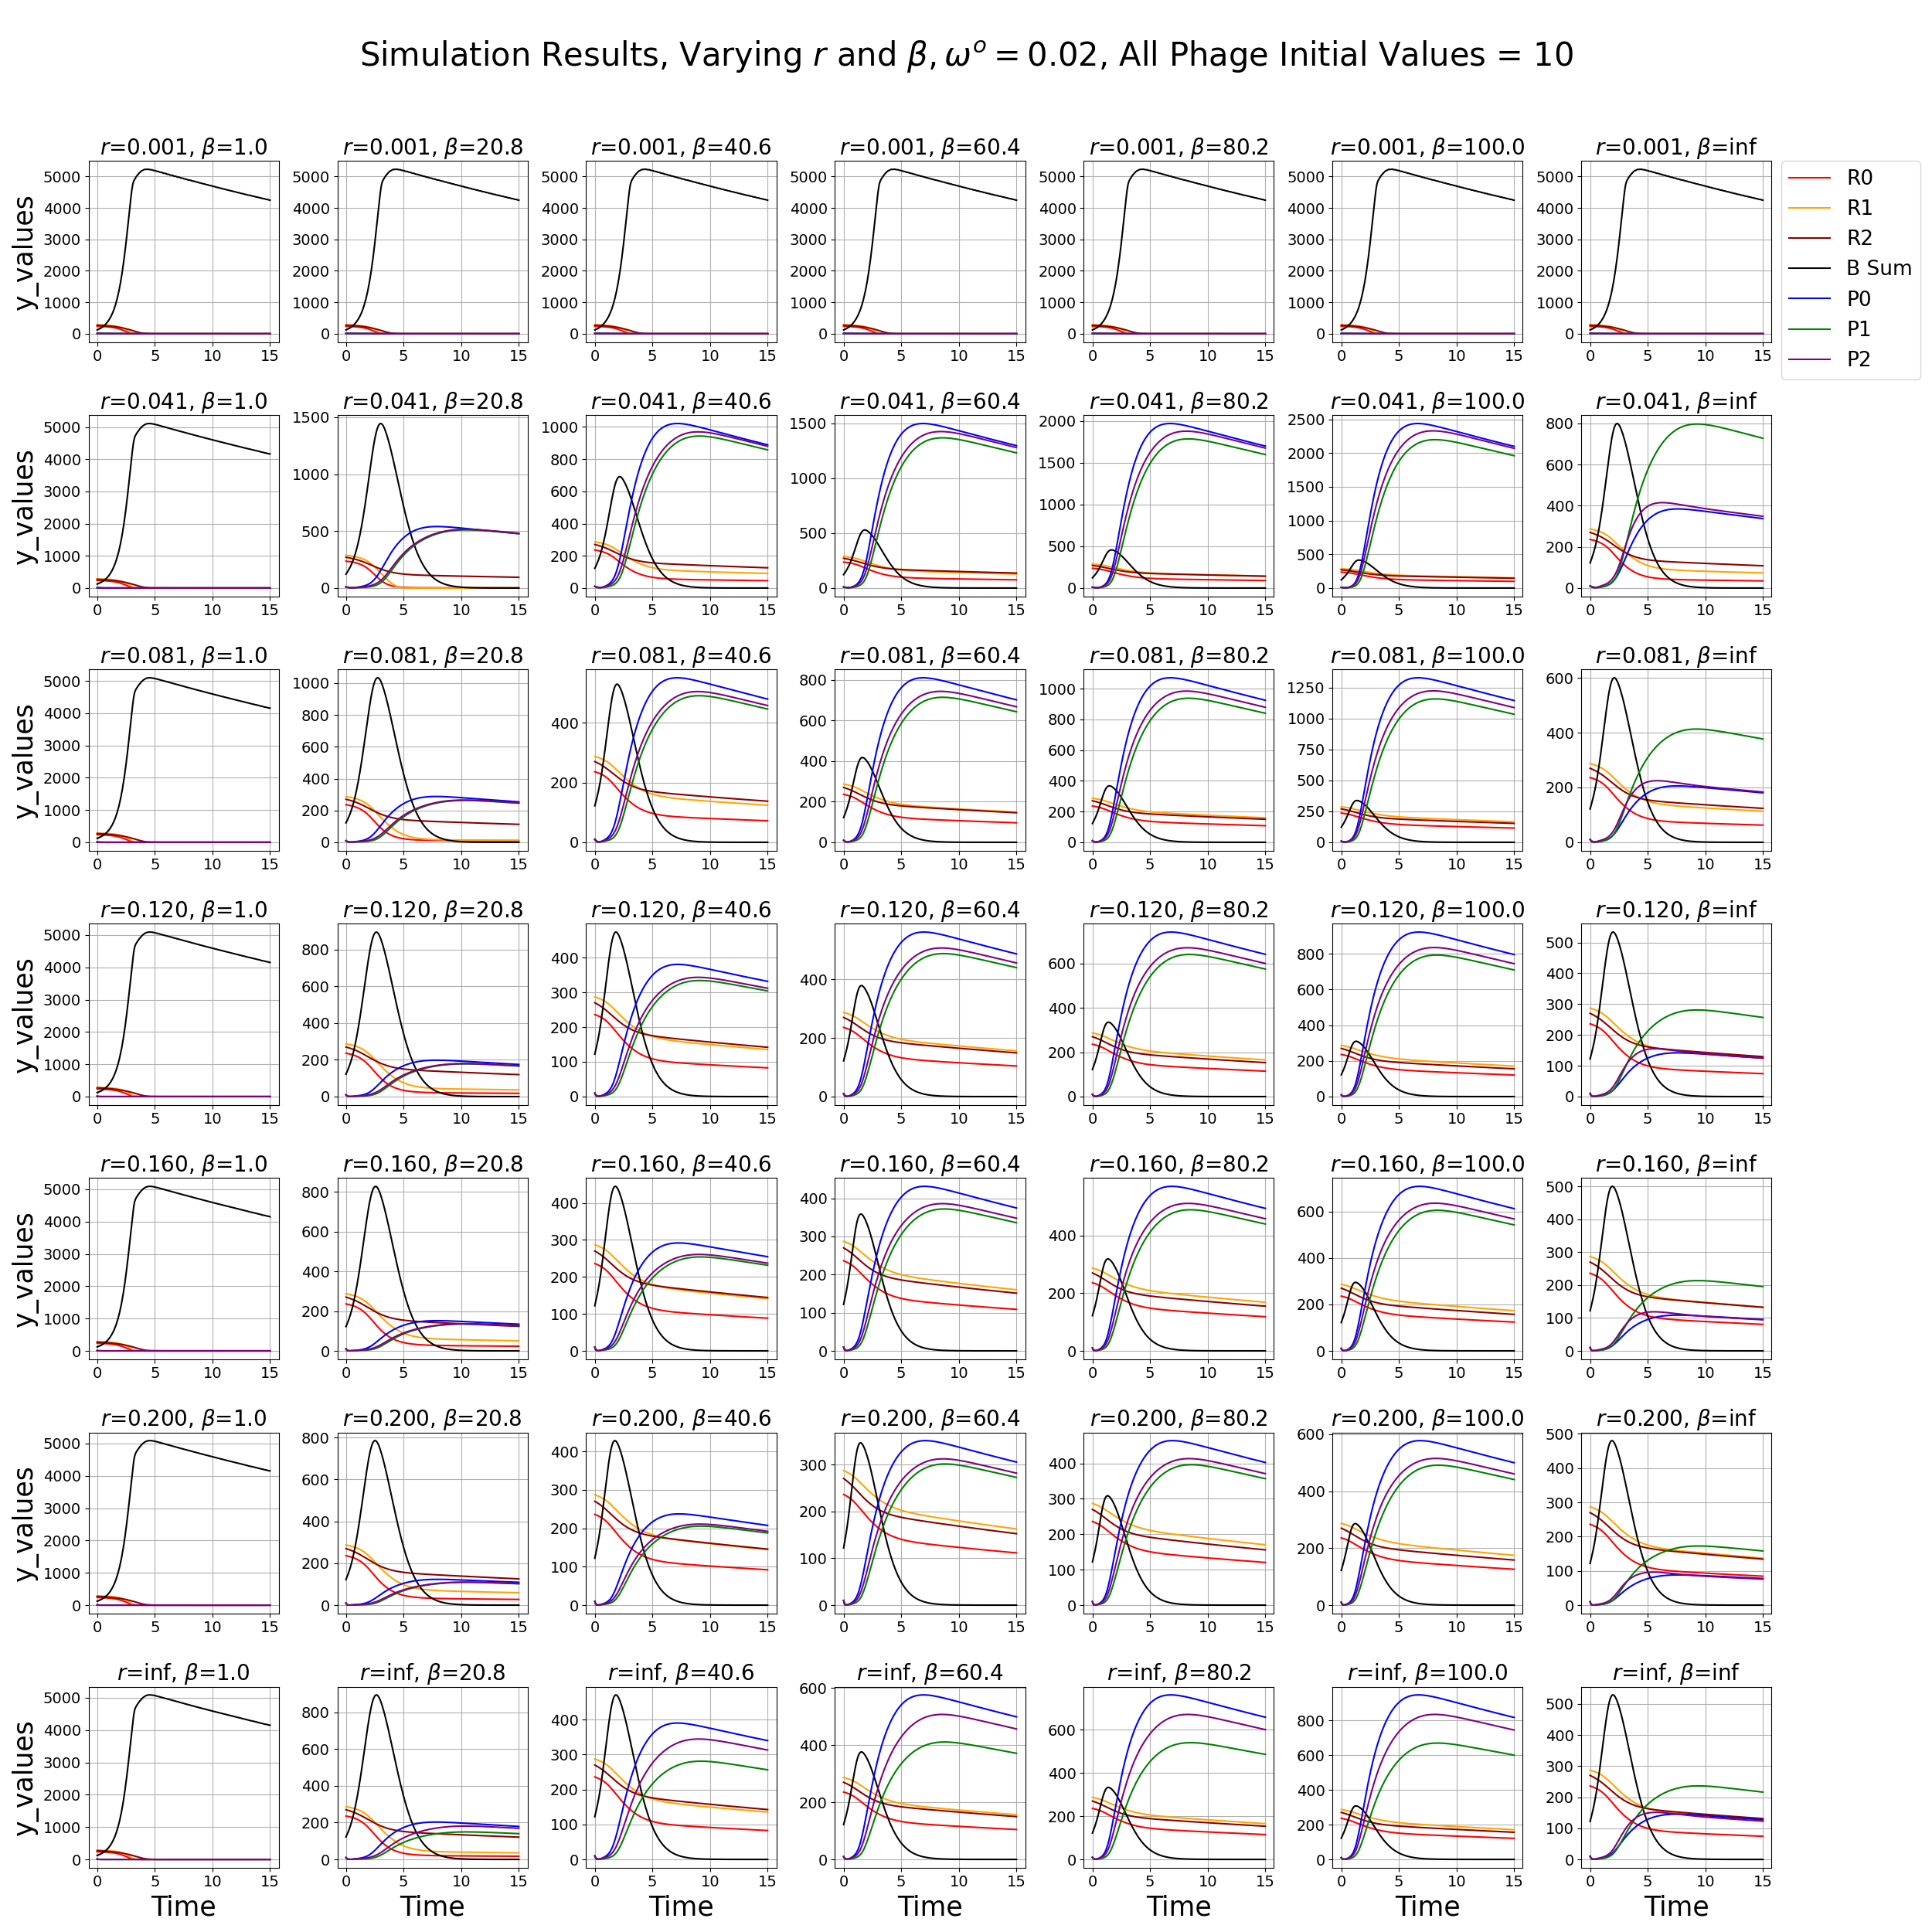
\includegraphics[width=\linewidth]{Plots/Created/UA/r_beta_washout_0.02.png}
        \caption{
            Washout $\omega^o=0.02$. 
        }
        \label{fig:created:r_beta_washout_0.02}
    \end{subfigure}
    \begin{subfigure}{0.49\linewidth}
        \centering
        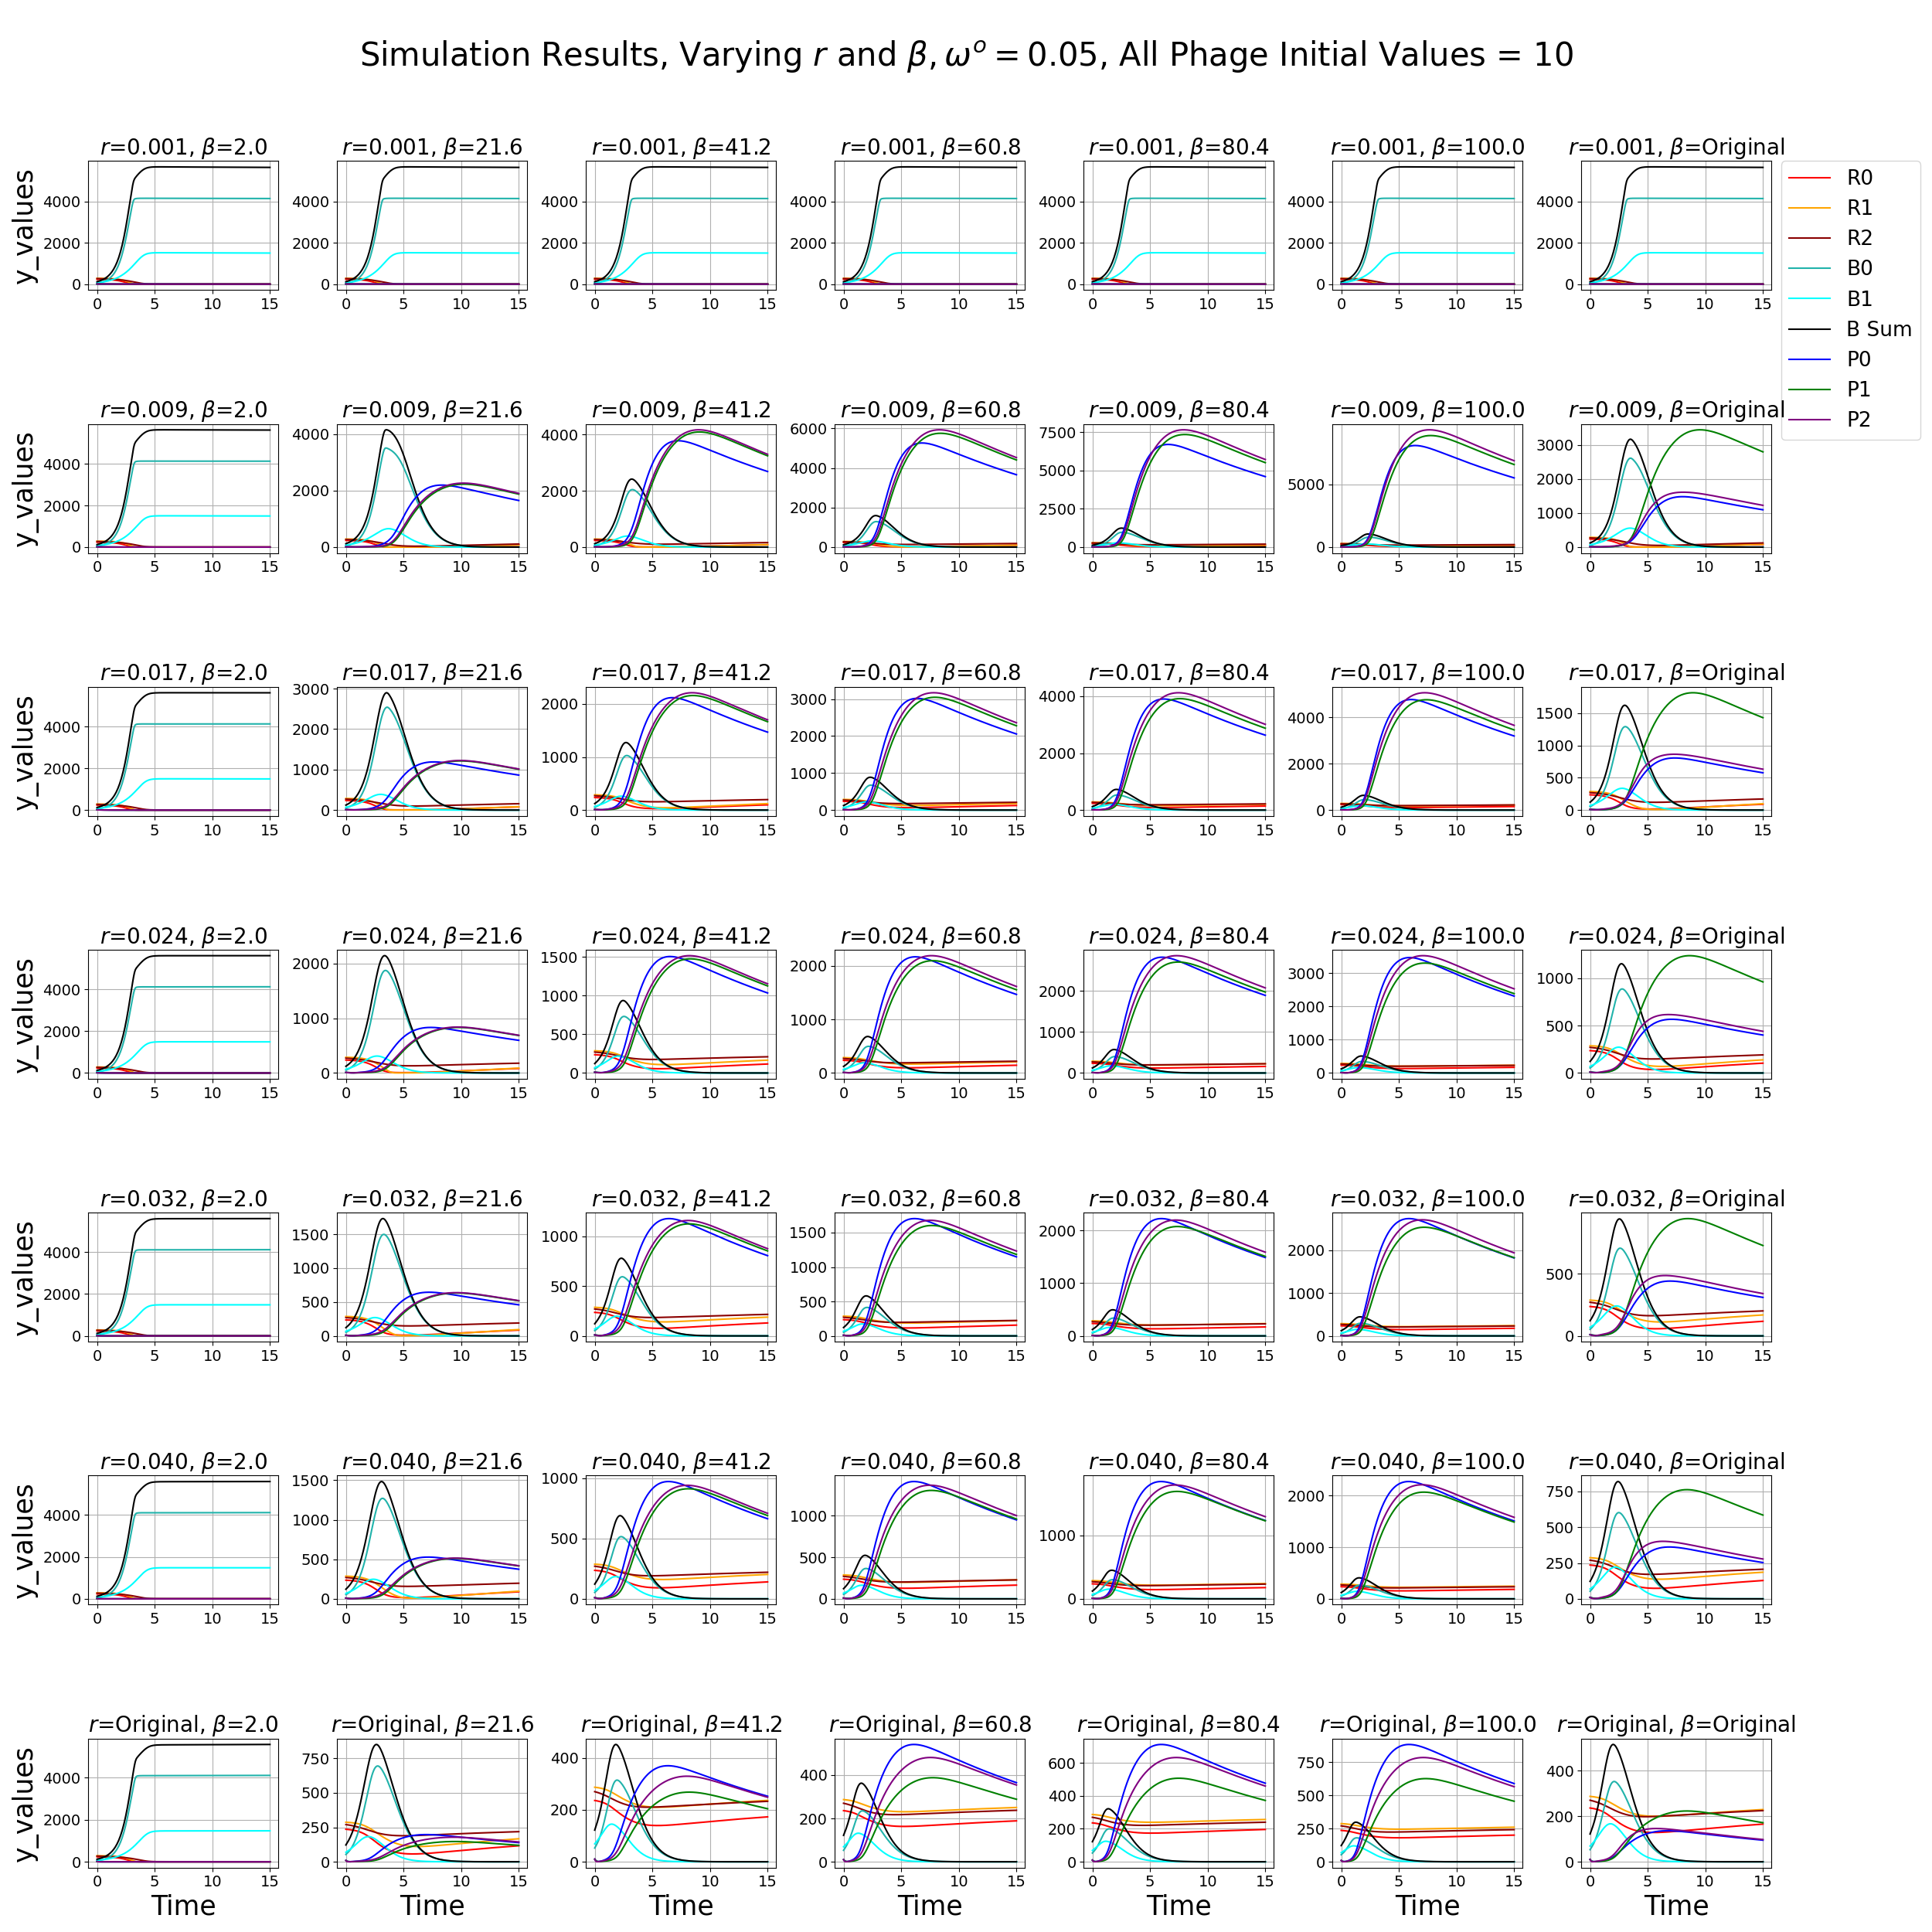
\includegraphics[width=\linewidth]{Plots/Created/UA/r_beta_washout_0.05.png}
        \caption{
            Washout $\omega^o=0.05$. 
        }
        \label{fig:created:r_beta_washout_0.05}
    \end{subfigure}
    \caption{
        Varying washout $\omega^o, r,$ and $\beta$. 
        The default values for the parameters can be found in \Cref{tab:appendixE:complex_model}. 
        All initial phage population values were set to 10. 
    }
\end{figure}

\section{Phage and Bacteria Survivability Analysis For A $20\times20\times10$ System}
In the context of large communities, it is important to understand how different conditions will influence if a phage or bacteria population will survive. 
Different interactions and environmental factors will influence how the community evolves. 
Sometimes populations of phages or bacteria will die out due to external factors, either that be a due to a lack of resources or bacteria to consume or infect, natural degradation, or external factors like UV light. 

Using the simulation framework, I created and analyzed a $20\times20\times10$ system using the extended Golding model. 
I selected two parameters, $\tau$ and $\beta$, to run a survivability analysis using the extended Golding model. 
A phage survived if its final population is greater than 1 at the end of the simulation. 
A bacteria population survived if the final population for the uninfected bacteria was greater than 1. 

Each phage is guaranteed to interact with at least one bacterium but no more than two bacteria. 
Each bacterium interacts with at least one phage and one resource, but not more than two phages and two resources. 
Every resource interacts with at least one bacterium, and at most three bacteria. 
The parameter values were randomly selected from a uniform distribution in the Sobol analysis value ranges (\Cref{tab:appendixE:Sobol_analysis_values}). 

\Cref{fig:created:survivability} shows the phage and bacteria survivability matrix. 
It appears as if there is an inverse relationship between phage and bacteria survivability. 
If the phages survived, the bacteria died out. 
If the bacteria survived, the phages did not survive. 
The phages only died out with small burst sizes, $\beta$, while otherwise would consistently survive. The small burst size ensured that the phages could not proliferate in time. 
Once the burst size became large enough, around $\beta = 3$, more than half of the phages were able to survive. 
The bacteria only survived with small burst sizes $\beta$. 
For large burst sizes, the phages would grow too fast and infect the bacteria. 

$\tau$ had less of an influence in survivability than $\beta$ did, except for when the $\beta$ values were less than 20. 
As $\tau$ increases, fewer phages survive and more bacteria survive. 
$\tau$ determines how fast a bacterium goes through the infection process, so as $\tau$ increases fewer phages will survive. 
The bacterium takes longer for the infection process to complete, so there is a greater chance for the phages and infected bacteria to be washed out before more phages can be created. 

For the most part, the competitive exclusion principle is respected. 
The majority of the simulations resulted in less than 10 uninfected bacteria surviving. 
For small burst sizes, there were more than 10 surviving bacteria, however if the simulation length were to be extended it would be expected that more bacteria populations will start to die out. 

\begin{figure}[]
    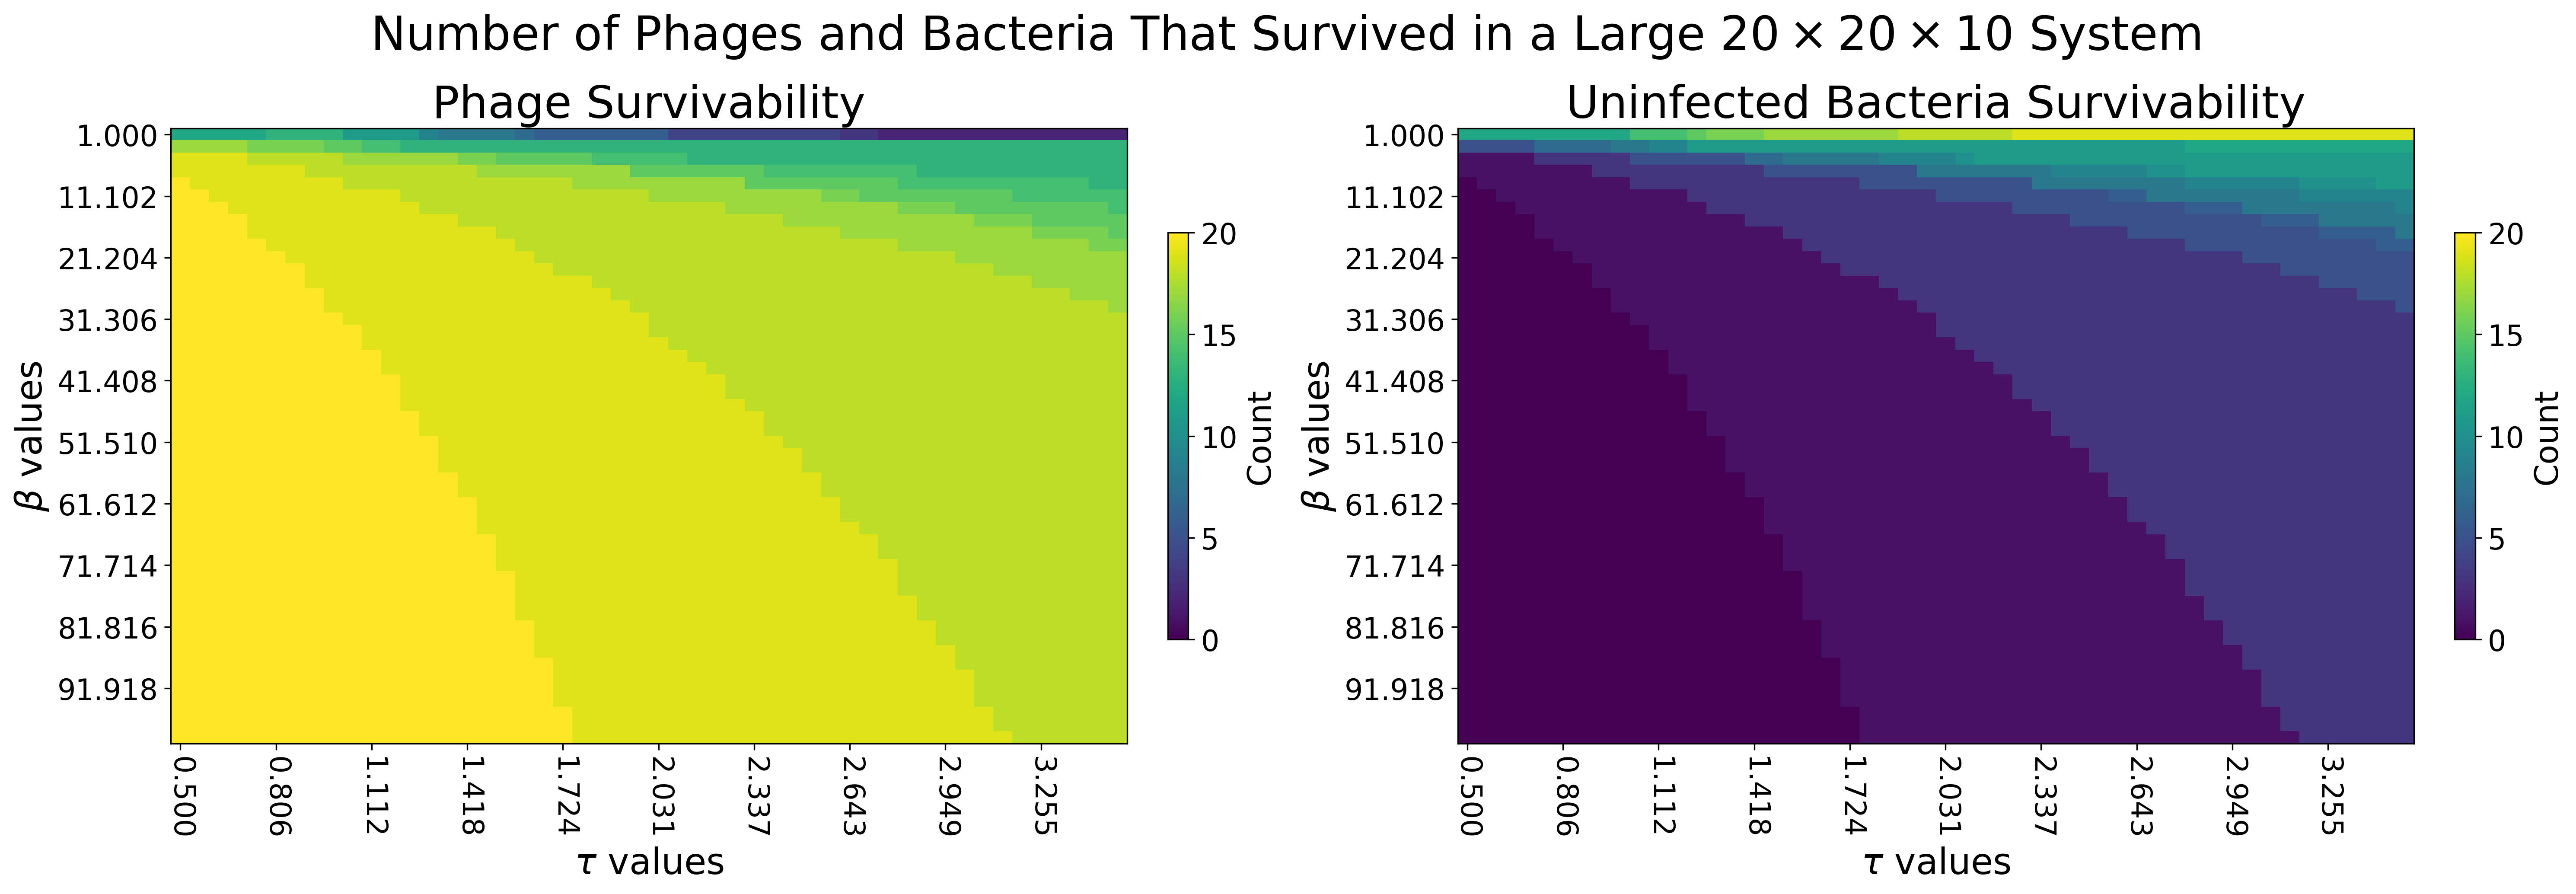
\includegraphics[width=1\textwidth]{Plots/Created/phage_bacteria_survivability.png}
    \centering
    \caption{
        The output graph for the default parameter values for a large $20\times 20 \times 10$ network. 
        Parameter values were randomly chosen in the interval given by \Cref{tab:appendixE:Sobol_analysis_values}. 
    \label{fig:created:survivability}
    }
\end{figure}